\documentclass[pdftex, letterpaper, 12pt, openany]{book}

\usepackage[spanish]{babel}
\usepackage{datetime}
\usepackage[colorlinks=true,linkcolor=black]{hyperref}
\usepackage[utf8x]{inputenc}
\usepackage[pdftex]{color,graphicx}
\usepackage[nottoc]{tocbibind}
\usepackage{babelbib}
\usepackage{natbib}
\usepackage{fullpage}
\usepackage{caption}
\usepackage{color, colortbl}
\usepackage{hyperref}
\usepackage{graphicx}
\usepackage{float}
\setcounter{tocdepth}{4}
\setcounter{secnumdepth}{4}
\restylefloat{table}
%\setlength{\parskip}{8mm}

%\setcounter{secnumdepth}{1}
\newcommand{\HRule}{\rule{\linewidth}{0.5mm}}
%\definecolor{cites}{rgb}{0,0,0}
\hypersetup{colorlinks=false, citecolor=cites}

\begin{document}

\frontmatter

\label{ch:portada}
\thispagestyle{empty}

\begin{figure}[!htb]
	\minipage{0.15\textwidth}
	\raggedright
	
\includegraphics[width=\linewidth]{img/ucv.jpg}
	\endminipage\hfill
	\minipage{0.15\textwidth}
	\raggedleft
	
\includegraphics[width=\linewidth]{img/ciens.jpg}
	\endminipage\hfill
\end{figure}

\begin{center}
	Universidad Central de Venezuela\\
	Facultad de Ciencias\\
	Escuela de Computación\\
	
\end{center}

\vspace{2.5cm}
\begin{center}
	\large{\textbf{ ESTUDIO DE UNA SOLUCIÓN PARA EL PROCESO DE INSPECCIÓN DE VEHÍCULOS EN UNA COMPAÑÍA DE SEGUROS. }}
\end{center}

\vspace{6.0cm}
\begin{center}
	Trabajo de Seminario \\
	presentado ante la Ilustre\\
	Universidad Central de Venezuela\\
	Por el Bachiller\\
	Ricardo Antonio Cerqueira Salazar\\
\end{center}

\begin{center}
	Tutor:\\ Prof. Franky Uzcategui\\
\end{center}

\vspace{1.0cm}
\begin{center}
	Caracas, \monthname[\month] de \the\year
\end{center}

\newpage

\tableofcontents
\listoffigures
\renewcommand{\listtablename}{\'Indice de tablas}
\renewcommand{\tablename}{Tabla}
\listoftables


\mainmatter

\chapter*{INTRODUCCIÓN}

\addcontentsline{toc}{chapter}{INTRODUCCIÓN}

\setlength{\parskip}{4mm}

En la actualidad el mercado asegurador venezolano se encuentra en una alta demanda. Debido a esto las empresas aseguradoras poseen un alto índice de clientes cuyo manejo de información es indispensable para dar un buen servicio.

El alto volumen de información manejada en la suscripción de vehículos de cada uno de los clientes genera un fuerte impacto administrativo, tanto de personal como de tiempo. Los peritos encargados de la inspección del los vehículos, diariamente manejan un gran volumen de planillas las cuales pueden llegar a traspapelarse.

Por lo cual se propone una solución computacional mediante la cual se plantea desarrollar una aplicación web que permitirá el almacenamiento de dichas planillas de suscripción, para llevar un mejor manejo de las mismas. Administrarlas en caso de una re-inspección y poder gestionar mejor tramites como: atención del cliente, suscripción al seguro e inspección del vehículo. Garantizando así un mejor desempeño y velocidad en la atención de los clientes generando así una mayor satisfacción para los mismos.

La estructura de este documento consiste de las siguientes secciones: El primer capitulo el Marco Teórico consiste de los conceptos y definiciones sobre los temas y tecnologías utilizadas para el desarrollo de este estudio. 

El segundo capitulo Marco Metodológico consta de las diferente metodologías tanto ágiles como tradicionales para el desarrollo de software. En este capitulo se plantearan las diferentes características entre ambas tecnologías mostrando sus ventajas y desventajas. Además se expondrá un cuadro comparativo en el cual se podrá establecer cual metodología es la mas conveniente a utilizar.

El tercer capitulo al ser una solución que abarca el peritaje de vehículos, se incluyen conceptos y términos asociados con el área de seguro, peritaje e inspecciones de vehículos.

Por ultimo en el cuarto capitulo se presenta la propuesta de Trabajo Especial de Grado, mostrando los objetivos que se desean logra al culminar, en conjunto con la propuesta de solución, su justificación y el alcance de la misma. Además se especificaran las diferentes tecnologías que se utilizaran para el desarrollo de la propuesta.
\setlength{\parskip}{0mm}
\chapter{Problema de Investigación}


\section{Situación actual} 



\section{Planteamiento del problema} 
\setlength{\parskip}{5mm}


Actualmente al asistir a la cita para la inspección del vehículo, el perito registra las especificaciones del mismo en una hoja para luego ser archivada y guardada, este proceso se realiza manualmente.

El procesos presenta una serie de inconveniente en cuando a la persistencia de los datos y la administración se refiere:

\begin{itemize}

	\item Las planillas de inspección se guardan solamente en físico.

	\item El riesgo de perder información que no esta respaldada.

	\item El acceso a la información, al ser una búsqueda manual, no es eficiente. 

\end{itemize}


Ante la situación descrita, se plantea elaborar una solución con tecnología Web, que permita a los peritos, mantener un registro digital de las planillas de inspección de los vehículos.



% Recibirá mediante un web service la información de la planilla y que esta pueda ser editada una vez antes de aceptar y guardarla en el sistema

% Mantener este registro de forma sistematizada 

% Actualmente al asistir a la cita para la inspección del vehiculo, se anotan las especificaciones del mismo en una hoja para luego ser pasada a la computadora, este proceso ocasiona gastos de recursos tanto del personal encargado de traspasar la informacion  como insumos como hojas entre otras  

% Recibirá mediante un web service la información de la planilla y que esta pueda ser editada una vez antes de aceptar y guardarla en el sistema

\setlength{\parskip}{0mm}


% diagrama y arquitectura



\section{Justificación} 
\setlength{\parskip}{5mm}

Un sistema con tecnologías web, es la mejor solución para sistematizar la administración de las planillas de inspección y para el almacenamiento de las mismas de forma digital, para que de esta forma la empresa aseguradora pueda llevar un registro cuyo gestión sea mas eficiente y de múltiple acceso.

La implementación de este sistema representa una reducción riesgos y costos a largo plazo para la compañía, permitiendo que la gestión de las planillas de inspección y los procesos vinculados con ellas se lleven acabo de manera óptima.
\setlength{\parskip}{0mm}

\section{Objetivo general} 

Desarrollar una solución para el proceso de inspección de vehículos en una compañía de seguros.


\section{Objetivos específicos}

\begin{itemize}

	
	
	% \item Permitir la edición de la solicitudes de inscripción mediante la aplicación web.
	% \item Análisis y levantamiento de información.

	% \item Diseñar prototipos.

	% \item Diseñar la base de datos.

	% \item Diseñar interfaces de la aplicación web.

	% \item Implementar funcionalidades del sistema.
	% % \item Diseñar e implementar un sistema de registro.

   \item Análisis de especificaciones del proceso de inspección de vehículos para suscripción

   \item Diseño del modelo de datos, de las interfaces y de los componentes de los módulos del sistema

   \item Desarrollo del sistema

   \item Pruebas funcionales y de usabilidad
	
	

\end{itemize}





\section{Alcance}

Como alcance del trabajo especial de grado se tiene previsto lograr el registro de usuarios que accederán al sistema para gestionar las planillas, la captura de los datos de la planilla de inspección, la edición de la planilla en caso de incongruencias antes de ser almacenada y guardar el conjunto de datos en la base de datos para su posterior consulta


\chapter{Marco Conceptual}

\section{Sistema de información} 	
\setlength{\parskip}{5mm}
Los SI son conjuntos organizados de elementos dirigidos a recoger, procesar, almacenar y distribuir información de manera que pueda ser utilizada por las personas adecuadas dentro de las empresas, de modo que desempeñen sus actividades de manera eficaz y eficiente” (Colomina, 1998)

Desde el punto de vista empresarial, los sistemas de información tienen como propósito perfeccionar las actividades llevadas a cabo en una organización, y así alcanzar ventajas competitivas.

\setlength{\parskip}{0mm}


\section{Tipos de sistemas de información} 	

\subsection{Sistema de procesamiento de transacciones (TPS)}
\setlength{\parskip}{5mm}
Cuando un sistema recopila, almacena y altera la información creada a partir de transacciones llevadas a cabo dentro de una organización se denomina sistema de procesamiento de transacciones. Tiene como finalidad procesar las transacciones diarias de una empresa, acumulando toda la información recibida en una base de datos para su posterior consulta.

\setlength{\parskip}{0mm}

\subsection{Sistema de información gerencial (MIS)}
\setlength{\parskip}{5mm}
Un sistema de información gerencial es aquel utilizado por la empresa para solventar inconvenientes en la misma. Es decir, el objetivo del mismo es la suministración de información para la resolución de problemas a través de la interacción entre tecnologías y personas.

Los datos aportados por el sistema deben disponer de cuatro cualidades elementales: calidad, oportunidad, cantidad y relevancia.

\setlength{\parskip}{0mm}

\subsection{Sistema de apoyo a la toma de decisiones (DSS)}
\setlength{\parskip}{5mm}

Este sistema se basa en el estudio y la comparación entre un conjunto de variables con el objeto de contribuir a la toma de decisiones dentro de una empresa. El apoyo dado por el sistema involucra la estimación, valoración y balance entre alternativas. Al igual que el sistema de información gerencial, esta tecnología interacciona con personas en el filtrado de información que permite optar por la decisión mas acertada.


% Las principales características de estos son:

%     Suelen introducirse después de haber implantado los Sistemas Transaccionales más relevantes de la empresa, ya que estos últimos constituyen su plataforma de información.

%     La información que generan sirve de apoyo a los mandos intermedios y a la alta administración en el proceso de toma de decisiones.

% Suelen ser intensivos en cálculos y escasos en entradas y salidas de información. Así, por ejemplo, un modelo de planeación financiera requiere poca información de entrada, genera poca información como resultado, pero puede realizar muchos cálculos durante su proceso.

%     No suelen ahorrar mano de obra. Debido a ello, la justificación económica para el desarrollo de estos sistemas es difícil, ya que no se conocen los ingresos del proyecto de inversión.

%     Suelen ser Sistemas de Información interactivos y amigables, con altos estándares de diseño gráfico y visual, ya que están dirigidos al usuario final.

%     Apoyan la toma de decisiones que, por su misma naturaleza son repetitivos y de decisiones no estructuradas que no suelen repetirse. Por ejemplo, un Sistema de Compra de Materiales que indique cuándo debe hacerse un pedido al proveedor o un Sistema de Simulación de Negocios que apoye la decisión de introducir un nuevo producto al mercado.

%     Estos sistemas pueden ser desarrollados directamente por el usuario final sin la participación operativa de los analistas y programadores del área de informática.

% Este tipo de sistemas puede incluir la programación de la producción, compra de materiales, flujo de fondos, proyecciones financieras, modelos de simulación de negocios, modelos de inventarios, entre otros.


% https://richardunefa.wordpress.com/principios-de-sistemas-de-informacion/

\setlength{\parskip}{0mm}

\subsection{Sistema de información ejecutiva (EIS)}
\setlength{\parskip}{5mm}
 Esta tecnología es utilizada por los gerentes de una empresa, ya que permite acceder a la información interna y externa de la misma, disponiendo de los datos que puedan llegar a afectar su buen rendimiento.
De esta manera, el ejecutivo podrá conocer el estado de todos los indicadores, incluso aquellos que no cumplan con las expectativas y a partir de esto, tomar las medidas que considere adecuadas.
\setlength{\parskip}{0mm}


% http://www.tiposde.org/informatica/89-tipos-de-sistemas-de-informacion/
% http://www.monografias.com/trabajos7/sisinf/sisinf2.shtml


\section{Base de Datos} 	
\setlength{\parskip}{5mm}
Una base de datos (cuya abreviatura es BD) es una entidad en la cual se pueden almacenar datos de manera estructurada, con la menor redundancia posible. Diferentes programas y diferentes usuarios deben poder utilizar estos datos. Por lo tanto, el concepto de base de datos generalmente está relacionado con el de red ya que se debe poder compartir esta información. De allí el término base. Sistema de información es el término general utilizado para la estructura global que incluye todos los mecanismos para compartir datos que se han instalado. (\citet{bdbib}, 2016) 


\setlength{\parskip}{0mm}



\subsection{Sistema Manejador de Base de Datos}
\setlength{\parskip}{5mm}
Un sistema manejador de bases de datos (SGBD, por sus siglas en inglés) o DataBase Management System (DBMS) es una colección de software muy específico, cuya función es servir de interfaz entre la base de datos, el usuario y las distintas aplicaciones utilizadas.

Como su propio nombre indica, el objetivo de los sistemas manejadores de base de datos es precisamente el de manejar un conjunto de datos para convertirlos en información relevante para la organización, ya sea a nivel operativo o estratégico.
 
Lo hace mediante una serie de rutinas de software para permitir su uso de una manera segura, sencilla y ordenada. Se trata, en suma, de un conjunto de programas que realizan tareas de forma interrelacionada para facilitar la construcción y manipulación de bases de datos, adoptando la forma de interfaz entre éstas, las aplicaciones y los mismos usuarios. (\citet{smdbbib}, 2015)

El SMDB puede dividirse en tres subsistemas:
\setlength{\parskip}{0mm}
\begin{itemize}

    \item El sistema de administración de archivos: para almacenar información en un medio físico
    
    \item El DBMS interno: para ubicar la información en orden
    
    \item El DBMS externo: representa la interfaz del usuario

\end{itemize}



\setlength{\parskip}{5mm}
A continuación se presentarán algunos ejemplos de SMBD.
\setlength{\parskip}{0mm}

\subsection {PostgresSQL}
\setlength{\parskip}{5mm}
PostgreSQL es un sistema de gestión de bases de datos objeto-relacional, distribuido bajo licencia BSD y con su código fuente disponible libremente. Es el sistema de gestión de bases de datos de código abierto más potente del mercado.

PostgreSQL utiliza un modelo cliente/servidor y usa multi-procesos en vez de multi-hilos para garantizar la estabilidad del sistema. Un fallo en uno de los procesos no afectará el resto y el sistema continuará funcionando.

Sus características técnicas la hacen una de las bases de datos más potentes y robustas del mercado. Su desarrollo comenzó hace más de 16 años, y durante este tiempo, estabilidad, potencia, robustez, facilidad de administración e implementación de estándares han sido las características que más se han tenido en cuenta durante su desarrollo.

PostgreSQL funciona muy bien con grandes cantidades de datos y una alta concurrencia de usuarios accediendo a la vez a el sistema. (\citet{postgresbib}, 2011)
\setlength{\parskip}{0mm}


%\url{http://www.postgresql.org.es/sobre_postgresql}
\newpage
\subsection{MySQL}
\setlength{\parskip}{5mm}
MySQL es un sistema de administración de bases de datos (Database Management System, DBMS) para bases de datos relacionales. Así, MySQL no es más que una aplicación que permite gestionar archivos llamados de bases de datos.

MySQL, como base de datos relacional, utiliza múltiples tablas para almacenar y organizar la información. MySQL fue escrito en C y C++ y destaca por su gran adaptación a diferentes entornos de desarrollo, permitiendo su interacción con los lenguajes de programación más utilizados como PHP, Perl y Java y su integración en distintos sistemas operativos.

También es muy destacable, la condición de open source de MySQL, que hace que su utilización sea gratuita e incluso se pueda modificar con total libertad, pudiendo descargar su código fuente. Esto ha favorecido muy positivamente en su desarrollo y continuas actualizaciones, para hacer de MySQL una de las herramientas más utilizadas por los programadores orientados a Internet.
\setlength{\parskip}{0mm}
(\citet{mysqlbib}, 2005)
%http://www.esepestudio.com/noticias/que-es-mysql

\subsection{Oracle}
\setlength{\parskip}{5mm}
Oracle la Primera Base de Datos Diseñada para Grid Computing, es un sistema de gestión de base de datos relacional fabricado por Oracle Corporation. Oracle es básicamente un herramienta cliente/servidor para la gestión de base de datos la gran potencia que tiene y su elevado precio hace que solo se vea en empresas muy grandes y multinacionales, por norma general. Oracle Corporation :es una de las mayores compañías de software del mundo. Sus productos van desde bases de datos (Oracle) hasta sistemas de gestión. Cuenta además, con herramientas propias de desarrollo para realizar potentes aplicaciones, como Oracle Designer

Desarrollado sobre Oracle Database, Oracle Content Database ha sido diseñada para que las organizaciones puedan controlar y gestionar grandes volúmenes de contenidos no estructurados en un único repositorio con el objetivo de reducir los costes y los riesgos asociados a la pérdida de información.
\setlength{\parskip}{0mm}
(\citet{oraclebib}, 2014) 


\newpage
\subsection{Cuadro Comparativo SMBD}
\begin{table}[H]	
\begin{center}
\begin{tabular}{ | m{3cm} | m{4.5cm}| m{4.5cm}| } 
 \hline
 SMDB & Ventajas & Desventajas \\
 \hline
 PostgresSQL 
 &
 %ventajas
 - Multiplataforma.
 \newline
 - Diseñado para ambientes de alto volumen.
 \newline
 - Herramientas gráficas de diseño y administración.
 \newline
 - Tiene mejor soporte que los proveedores comerciales.
 \newline
 - Licencia abierta.
 &
 %desvantajas \\
-La sintaxis de algunos de sus comandos o sentencias no es nada intuitiva.
\newline
-Es más lento en inserciones y actualizaciones, ya que cuenta con cabeceras de intersección que no tienen otros SMBD.
\newline
-El soporte es en línea.
\\
  \hline
 MySQL
 &
 %ventajas
 - Tiene una mayor velocidad al realizar operaciones.
  \newline
 - Baja probabilidad de corromper datos.
  \newline
 - Característica única puede agrupar transacciones.
  \newline
 - Permite la gestión de diferentes usuarios y permisos.
  \newline
 - Es Licencia abierta.
 &
 %desvantajas
 -Un gran porcentaje de las utilidades de MySQL no están documentadas.
 \newline
 -Poco intuitivo.
 \\
 \hline
 Oracle
 &
 %ventajas
 - Es considerado como uno de los sistemas gestores de bases de datos más completo.
  \newline
 - Permite el uso de particiones.
  \newline
 - Consultas en paralelo.
  \newline
 - Las herramientas de configuración de Oracle son tal vez las mejores en el mercado.
 &
 %desvantajas
 
 - Un Oracle mal configurado puede ser desesperadamente lento.
  \newline
  - Es privativo, costos no muy asequibles.
 \\
 \hline
 \end{tabular}
\caption{Tabla comparativa de los Sistemas Manejadores de Base de Datos}
\label{Tabla:3}
\end{center}
\end{table}	

\newpage
%https://iessanvicente.com/colaboraciones/oracle.pdf

%%%%%%%%%%%%%%%%%%%%%%%% MOVIL %%%%%%%%%%%%%%%%%%%%%%%%%%%%%%%

	% \section{Base de datos móvil} 		

	% Es una Base de datos donde los usuarios pueden acceder a la información lejos de donde se encuentra almacenada la base de datos, se hace utilizando una conexión inalámbrica. (\citet{bdmovil}, 2012)

	% \subsection{Sistema manejador de base de datos móvil} 

	% \subsubsection{SQLite}
	% \setlength{\parskip}{5mm}


	% SQLite es una herramienta de software libre, que permite almacenar información en dispositivos empotrados de una forma sencilla, eficaz, potente, rápida y en equipos con pocas capacidades de hardware, como puede ser una PDA o un teléfono celular. SQLite implementa el estándar SQL92 y también agrega extensiones que facilitan su uso en cualquier ambiente de desarrollo. 

	% Esto permite que SQLite soporte desde las consultas más básicas hasta las más complejas del lenguaje SQL, y lo más importante es que se puede usar tanto en dispositivos móviles como en sistemas de escritorio, sin necesidad de realizar procesos complejos de importación y exportación de datos, ya que existe compatibilidad al 100\% entre las diversas plataformas disponibles, haciendo que la portabilidad entre dispositivos y plataformas sea transparente. (\citet{sqlitebib}, 2007)

	% Características:
	% \setlength{\parskip}{0mm}
	% \begin{itemize}

	% \item La base de datos completa se encuentra en un solo archivo.

	% \item Puede funcionar enteramente en memoria, lo que la hace muy rápida.

	% \item Tiene un footprint menor a 230KB.

	% \item Es totalmente auto-contenida (sin dependencias externas).

	% \item Cuenta con librerías de acceso para muchos lenguajes de programación.

	% \item Soporta texto en formato UTF-8 y UTF-16, así como datos numéricos de 64 bits.

	% \item Soporta funciones SQL definidas por el usuario (UDF).

	% \item El código fuente es de dominio público y se encuentra muy bien documentado.

	% \end{itemize}


	% \subsubsection{SYBASE}
	% \setlength{\parskip}{5mm}
	% Es la abreviatura de "Adaptive Server Enterprise", el software de base de datos relacional fabricado y vendido por Sybase Inc. ASE es un software versátil, de clase empresarial RDBMS que es especialmente bueno en el manejo de cargas de trabajo OLTPASE, es utilizado de forma intensiva en el mundo financiero (bancos, bolsas de valores, compañías de seguros), en el comercio electrónico, así como en el área de prácticamente todos los demás. (\citet{sybasebib}, 2011)

	% Características:
	% \setlength{\parskip}{0mm}

	% \begin{itemize}

	% \item La opción IMD permite la virtualización y crecimiento de datos fundamental para satisfacer las necesidades de grandes volúmenes de datos y organizaciones con alta concurrencia de usuarios.

	% \item Permite a los clientes existentes de Sybase ASE adoptar fácilmente las nuevas características y optimizaciones sin la necesidad de una actualización de la base de datos

	% \item Copias de respaldo en línea y de alto rendimiento. 

	% \item Soporte a múltiples herramientas de desarrollo y lenguajes de programación, como PowerBuilder, Visual Basic, Java, PHP.

	% \item Técnicas de particionamiento semántico de tablas que aumentan la velocidad de acceso a los datos. 

	% \end{itemize}


	% \subsubsection{MICROSOFT SQL SERVER CE}
	% \setlength{\parskip}{5mm}

	% Microsoft SQL Server Compact en su actual versión 4.0 es una base de datos compacta para aplicaciones de escritorio y web. SQL Server Compact 4.0 posee un modelo de programación común a otras ediciones de SQL Server para el desarrollo tanto de aplicaciones nativas como administradas. SQL Server Compact ofrece funcionalidad de base de datos relacional en un espacio reducido: un sólido almacén de datos, un procesador de consultas de optimización y una conectividad confiable y escalable. (\citet{sqlservercebib}, 2016) 

	% Características:
	% \setlength{\parskip}{0mm}

	% \begin{itemize}

	% \item Integración con WebMatrix una pila de desarrollo web gratuita que integra un servidor web con marcos de trabajo de programación y base de datos.

	% \item SQL Server Compact 4.0 usa el algoritmo SHA2 para proteger los datos y proporcionar un alto nivel de seguridad. 

	% \item SqlServerCe está enfocado a funcionar sobre dispositivos con características limitadas

	% \item Posee un motor de base de datos así como un procesador y un optimizador de consultas especialmente diseñado para entornos móviles

	% \item Únicamente soporta tipos de datos de cadena compatibles con Unicode (nchar, nvarchar, ntext). 

	% \end{itemize}

	% (\citet{sqlserverce2bib}, 2016)

	% \subsection{Arquitectura de una base de datos móvil} 

	% %\begin{figure}[H]
	% %\begin{center}
	% %	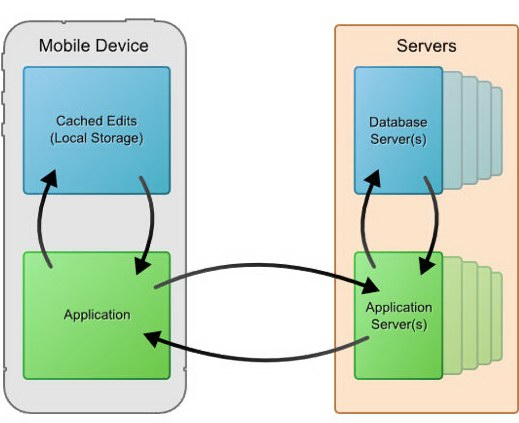
\includegraphics[width=13cm,height=8cm]{img/mobiledb.jpg}
	% %\end{center}
	% %\caption{Mobile divice. (Tomada de , 2014)}
	% %\label{fig:Mobiledb}
	% %\end{figure}



	% \section{Dispositivo móvil}
	% \setlength{\parskip}{5mm}
	% Dispositivo móvil (mobile device), también conocido como computadora de bolsillo o computadora de mano (palmtop o handheld), es un tipo de computadora de tamaño pequeño, con capacidades de procesamiento, con conexión a Internet, con memoria, diseñado específicamente para una función, pero que pueden llevar a cabo otras funciones más generales.

	% Estrictamente hablando, muchos de los llamados dispositivos móviles no tienen la capacidad de moverse. Más bien son dispositivos que pueden ser fácilmente transportados por sus usuarios
	% \setlength{\parskip}{0mm}

	% %Referecia
	% %↑ The University of California, Riverside, ed. (3 de diciembre de 2015). «When Apps Talk Behind Your Back» (en inglés). Consultado el 10 de diciembre de 2015. «We focused on a relatively neglected aspect of security research, which is the potential for good apps to leak personal information through the sites they interact with.»

	% \subsection{Tipos de dispositivos móviles}

	% \subsubsection{Teléfono Celular} 
	% \setlength{\parskip}{5mm}
	% Es un dispositivo inalámbrico electrónico que permite tener acceso a la red de telefonía celular o móvil. Se denomina celular debido a las antenas repetidoras que conforman la red, cada una de las cuales es una célula, si bien existen redes telefónicas móviles satelitales. Su principal característica es su portabilidad, que permite comunicarse desde casi cualquier lugar. Aunque su principal función es la comunicación de voz, como el teléfono convencional, su rápido desarrollo ha incorporado otras funciones como son cámara fotográfica, agenda, acceso a internet, reproducción de video e incluso GPS y reproductor mp3.

	% La comunicación telefónica es posible gracias a la interconexión entre centrales móviles y públicas. Según las bandas o frecuencias en las que opera el móvil, podrá funcionar en una parte u otra del mundo. La telefonía móvil consiste en la combinación de una red de estaciones transmisoras-receptoras de radio (repetidores, estaciones base o BTS) y una serie de centrales telefónicas de conmutación de 1.º y 5.º nivel (MSC y BSC respectivamente), que posibilita la comunicación entre terminales telefónicos portátiles (teléfonos móviles) o entre terminales portátiles y teléfonos de la red fija tradicional.
	% \setlength{\parskip}{0mm}
	% (\citet{celbib}, 2016)
	% %http://www.ecured.cu/Tel%C3%A9fono_celular

	% \subsubsection{Teléfonos Inteligentes}
	% \setlength{\parskip}{5mm}
	% Es un tipo de teléfono móvil construido sobre una plataforma informática móvil, con mayor capacidad de almacenar datos y realizar actividades, semejante a la de una minicomputadora, y con una mayor conectividad que un teléfono móvil convencional. El término «inteligente», que se utiliza con fines comerciales, hagan referencia a la capacidad de usarse como un computador de bolsillo, y llega incluso a reemplazar a una computadora personal en algunos casos.
	% (\citet{},2016)
	% \setlength{\parskip}{0mm}
	% \subsubsection{Tablets}
	% \setlength{\parskip}{5mm}
	% Es un dispositivo electrónico que tiene un tamaño intermedio entre el ordenador y el móvil. Sus características principales son las siguientes: su ligereza, su manejo intuitivo utilizando las manos, su elevada autonomía de uso y la no dependencia de otros accesorios complementarios.

	% Los sistemas operativos de estos dispositivos permiten una velocidad e inmediatez considerable, las aplicaciones que incorporan son muy accesibles y los procesos para su manejo son más rápidos que en los portátiles. Hay que tener presente que el tablet se maneja con las manos, probablemente la herramienta más dúctil y eficaz que existe (todavía las manos artificiales no han conseguido superar la destreza de las manos humanas).(\citet{tabletbib},2016)
	% \setlength{\parskip}{0mm}

	% %http://www.definicionabc.com/tecnologia/tablet.php


	% \section{Sistema Operativo Móvil}	
	% \setlength{\parskip}{5mm}
	% Un sistema operativo móvil o SO móvil es un sistema operativo que controla un dispositivo móvil al igual que los PCs que utilizan Windows o Linux, los dispositivos moviles tienen sus sistemas operativos como Android, IOS entre otros. Los sistemas operativos móviles son mucho más simples y están más orientados a la conectividad inalámbrica, los formatos multimedia para móviles y las diferentes maneras de introducir información en ellos.

	% Algunos de los sistemas operativos utilizados en los dispositivos móviles están basados en el modelo de capas.

	% \setlength{\parskip}{0mm}
	% \subsection{Tipos de sistemas operativos móviles}

	% \subsubsection{Android} 
	% \setlength{\parskip}{5mm}
	% Es un sistema operativo inicialmente pensado para teléfonos móviles, al igual que iOS, Symbian y Blackberry OS. Lo que lo hace diferente es que está basado en Linux, un núcleo de sistema operativo libre, gratuito y multiplataforma.

	% El sistema permite programar aplicaciones en una variación de Java llamada Dalvik. El sistema operativo proporciona todas las interfaces necesarias para desarrollar aplicaciones que accedan a las funciones del teléfono (como el GPS, las llamadas, la agenda, etc.) de una forma muy sencilla en un lenguaje de programación muy conocido como es Java
	% \setlength{\parskip}{0mm}
	% (\citet{androidbib}, 2016)
	% %t.xatakandroid.com/sistema-operativo/que-es-android

	% \subsubsection{iOS} 
	% \setlength{\parskip}{5mm}
	% Es un sistema operativo móvil desarrollado por Apple Inc. Inicialmente fue creado para el iPhone, pero con el tiempo fue adaptado para los demás dispositivos móviles de esta compañía (iPad y el iPod touch).

	% Este sistema operativo móvil está basado en el concepto de manipulación directa. Es decir, que el usuario puede interactuar directamente con la pantalla del dispositivo por medio de gestos multitáctiles como toques, pellizcos y deslices.
	% \setlength{\parskip}{0mm}
	% (\citet{iosbib}, 2016)


	% \subsubsection{Firefox OS}
	% \setlength{\parskip}{5mm}
	% Firefox OS (nombre clave: Boot to Gecko o B2G) es un sistema operativo móvil, basado en HTML5 con núcleo Linux, de código abierto para varias plataformas. Es desarrollado por Mozilla Corporation bajo el apoyo de otras empresas y una gran comunidad de voluntarios de todo el mundo. El sistema operativo está diseñado para permitir a las aplicaciones HTML5 comunicarse directamente con el hardware del dispositivo usando JavaScript y Open Web APIs.

	% Inicialmente estuvo enfocado en los dispositivos móviles, smartphones y tabletas, específicamente en el sector de gama baja, el 2 de julio de 2013, Telefónica comenzó la venta del primer terminal con Firefox OS, el ZTE Open.
	% \setlength{\parskip}{0mm}
	% (\citet{firefoxbib}, 2016)

	% %\section{Computación Móvil}	

	% %\subsection{Fases de la computación móvil}

	% %\subsection{Característica de la computación móvil}

	% \section{Aplicación Móvil}	

	% \subsection{Tipos de aplicaciones móviles}

	% \subsubsection{Aplicaciones Nativas}
	% \setlength{\parskip}{5mm}
	% Una aplicación nativa es la que se desarrolla de forma específica para un determinado  sistema operativo, llamado Software Development Kit o SDK. Cada una de las plataformas, Adroid, iOS o Windows Phone, tienen un sistema diferente, por lo que si quieres que tu app esté disponible en todas las plataformas se deberán de crear varias apps con el lenguaje del sistema operativo seleccionado.
	% Por ejemplo:
	% \setlength{\parskip}{0mm}
	% \begin{itemize}

	% 	\item Las apps para iOS se desarrollan con lenguaje Objective-C
		
	% 	\item Las apps para Android se desarrollan con lenguaje Java
		
	% 	\item Las apps en Windows Phone se desarrollan en .Net

		
	% \end{itemize}
	% \setlength{\parskip}{5mm}
	% Cuando hablamos de desarrollo móvil casi siempre nos estamos refiriendo a aplicaciones nativas. La principal ventaja con respecto a los otros dos tipos, es la posibilidad de acceder a todas las características del hardware del móvil: cámara, GPS, agenda, dispositivos de almacenamiento y otras muchas. Esto hace que la experiencia del usuario sea mucho más positiva que con otro tipo de apps.

	% Además las aplicaciones nativas no necesitan conexión a internet para que funcionen.

	% La descarga e instalación de estas apps se realiza siempre a través de las tiendas de aplicaciones (app store de los fabricantes). Esto facilita el proceso de marketing y promoción que explicaremos en próximos posts y que es vital para dar visibilidad a una app.

	% Ventajas
	% \setlength{\parskip}{0mm}
	% \begin{itemize}

	% 	\item Acceso completo al dispositivo. 
		
	% 	\item Mejor experiencia del usuario. 
		
	% 	\item Visibilidad en APP Store.
		
	% 	\item Envió de notificaciones o avisos a los usuarios.
		
	% 	\item La actualización de la app es constante.
		
	% \end{itemize}

	% Inconvenientes

	% \begin{itemize}

	% 	\item Diferentes habilidades/ idiomas/ herramientas para cada plataforma de destino.

	% 	\item Tienden a ser mas caras de desarrollar. 

	% 	\item El código del cliente no es reutilizable entra las diferentes plataformas.
		
	% \end{itemize}

	% \subsubsection{Aplicaciones Web}
	% \setlength{\parskip}{5mm}
	% Una aplicación web o webapp es la desarrollada con lenguajes muy conocidos por los programadores, como es el HTML, Javascript y CSS. La principal ventaja con respecto a la nativa es la posibilidad de programar independiente del sistema operativo en el que se usará la aplicación. De esta forma se pueden ejecutar en diferentes dispositivos sin tener que crear varias aplicaciones.

	% Las aplicaciones web se ejecutan dentro del propio navegador web del dispositivo a través de una URL. Por ejemplo en Safari, si se trata de la plataforma iOS. El contenido se adapta a la pantalla adquiriendo un aspecto de navegación APP.

	% ¿Puede considerarse esto una APP? En realidad la gran diferencia con una aplicación nativa (además de los inconvenientes que se muestran en la tabla) es que no necesita instalación por lo que no pueden estar visibles en app store y la promoción y comercialización debe realizarse de forma independiente. De todas formas se puede crear un acceso directo que sería como “instalar” la aplicación en el dispositivo.

	% Las apps web móviles son siempre una buena opción si nuestro objetivo es adaptar la web a formato móvil.

	% Ventajas
	% \setlength{\parskip}{0mm}
	% \begin{itemize}

	% 	\item El mismo código base reutilizable en múltiples plataformas 
		
	% 	\item Proceso de desarrollo mas sencillo y económico 
		
	% 	\item No necesitan ninguna aprobación para publicarse ( a diferencia de las nativas para estar visibles en la app store)
		
	% 	\item El usuario siempre dispone de la ultima versión 
		
	% 	\item Pueden reutilizarse sitios "resposive" ya diseñados
		
	% \end{itemize}

	% Inconvenientes

	% \begin{itemize}

	% 	\item Inconvenientes
		
	% 	\item Requiere de conexión a internet
		
	% 	\item Acceso muy limitado a los elementos y características del hardware del dispositivo
		
	% 	\item La experiencia del usuario (navegación, interacción) y el tiempo de respuesta es menor en una app nativa
		
	% 	\item Requiere de mayor esfuerzo en promoción y visibilidad

	% \end{itemize}

	% \subsubsection{Aplicaciones Híbrida}

	% \setlength{\parskip}{5mm}
	% Una aplicación híbrida es una combinación de las dos anteriores, se podría decir que recoge lo mejor de cada una de ellas. Las apps híbridas se desarrollan con lenguajes propios de las webabpp, es decir, HTML, Javascript y CSS por lo que permite su uso en diferentes plataformas, pero también dan la posibilidad de acceder a gran parte de las características del hardware del dispositivo. La principal ventaja es que a pesar de estar desarrollada con HTML, Java o CSS, es posible agrupar los códigos y distribuirla en app store.


	% Ventajas
	% \setlength{\parskip}{0mm}
	% \begin{itemize}

	% 	\item Es posible distribuirla en las tiendas iOS y android 
		
	% 	\item Instalación nativa pero construida con JavaScript, HTML y CSS
		
	% 	\item El mismo código base para múltiples plataformas
		
	% 	\item Acceso a parte del hardware del dispositivo
		
	% \end{itemize}

	% Inconvenientes

	% \begin{itemize}

	% 	\item Experiencia del usuario mas propia de la aplicación web que de la app nativa
		
	% 	\item Diseño visual no siempre relacionado con el sistema operativo en el que se muestre.
		
	% \end{itemize}


	% (\citet{tipoaplicacionesmobilesbib}, 2014)
	% %https://www.lancetalent.com/blog/tipos-de-aplicaciones-moviles-ventajas-inconvenientes/
%%%%%%%%%%%%%%%%%%%%%%%% END MOVIL %%%%%%%%%%%%%%%%%%%%%%%%%%%


\section{Tecnologías de desarrollo web}

\subsection{HTML}

\setlength{\parskip}{5mm}

HTML, sigla en inglés de HyperText Markup Language (lenguaje de marcas de hipertexto), hace referencia al lenguaje de marcado para la elaboración de páginas web. Es un estándar que sirve de referencia del software que conecta con la elaboración de páginas web en sus diferentes versiones, define una estructura básica y un código (denominado código HTML) para la definición de contenido de una página web, como texto, imágenes, vídeos, juegos, entre otros. 

Los documentos HTML son descritos por las etiquetas HTML, cada etiqueta HTML describe diferentes contenidos de documentos.(\citet{htmlbib}, 2016)

\setlength{\parskip}{0mm}

\subsection{CSS}
\setlength{\parskip}{5mm}
Hoja de estilo en cascada o CSS (siglas en inglés de cascading style sheets) es un lenguaje usado para definir y crear la presentación de un documento estructurado escrito en HTML o XML . 

La idea que se encuentra detrás del desarrollo de CSS es separar la estructura de un documento de su presentación. Es usado para definir los estilos de nuestra pagina web, incluyendo diseño, layouts y una variedad de vistas en los diferentes dispositivos y sus tamaños de pagina. (\citet{cssbib}, 2016)
\setlength{\parskip}{0mm}

\subsection{JavaScript}
\setlength{\parskip}{5mm}
Javascript es un lenguaje de programación interpretado, dialecto del estándar ECMAScript. Se define como orientado a objetos, basado en prototipos, imperativo, débilmente tipeado y dinámico.

Se utiliza principalmente en su forma del lado del cliente, implementado como parte de un navegador web permitiendo mejoras en la interfaz de usuario y páginas web dinámicas aunque existe una forma de JavaScript del lado del servidor (Server-side JavaScript o SSJS). Su uso en aplicaciones externas a la web, por ejemplo en documentos PDF, aplicaciones de escritorio es también significativo.

Tradicionalmente se venía utilizando en páginas web HTML para realizar operaciones y únicamente en el marco de la aplicación cliente, sin acceso a funciones del servidor. Actualmente es ampliamente utilizado para enviar y recibir información del servidor junto con ayuda de otras tecnologías como AJAX. JavaScript se interpreta en el agente de usuario al mismo tiempo que las sentencias van descargándose junto con el código HTML.(\citeauthor{javascripbib}, \citeyear{javascripbib})
\setlength{\parskip}{0mm}


\subsection{JQuery}
\setlength{\parskip}{5mm}
jQuery es una biblioteca de JavaScript, creada inicialmente por John Resig, que permite simplificar la manera de interactuar con los documentos HTML, manipular el árbol DOM, manejar eventos, desarrollar animaciones y agregar interacción con la técnica AJAX a páginas web. Fue presentada el 14 de enero de 2006 en el BarCamp NYC. jQuery es la biblioteca de JavaScript más utilizada.

jQuery es software libre y de código abierto, posee un doble licenciamiento bajo la Licencia MIT y la Licencia Pública General de GNU v2, permitiendo su uso en proyectos libres y privados. jQuery, al igual que otras bibliotecas, ofrece una serie de funcionalidades basadas en JavaScript que de otra manera requerirían de mucho más código, es decir, con las funciones propias de esta biblioteca se logran grandes resultados en menos tiempo y espacio.
\setlength{\parskip}{0mm}
(\citet{jquerybib}, 2009)
%http://www.desarrolloweb.com/articulos/introduccion-jquery.html

\subsection{JQueryUI}
\setlength{\parskip}{5mm}
jQuery UI es un complemento que permite implementar componentes diversos para generar interfaces de usuario en páginas web, además de otras funcionalidades básicas para crear aplicaciones web enriquecidas. Como su propio nombre indica, está basado en el popular framework Javascript y podemos encontrar links, explicaciones, así como demos y descargas a partir del sitio web oficial de jQuery.

Es una biblioteca de componentes y cada componente o módulo se desarrolla de acuerdo a la filosofía de jQuery (find something, manipulate it: encuentra algo, manipúlalo).
\setlength{\parskip}{0mm}
(\citet{jqueryuibib}, 2013)
%http://www.desarrolloweb.com/manuales/manual-jqueryui.html

\subsection{Boopstrap}
\setlength{\parskip}{5mm}
Bootstrap o twitter-bootstrap es un framework creado originalmente por dos desarrolladores/diseñadores de twitter para acelerar el diseño de nuevas aplicaciones web.
El framework proporciona clases css y código javascript para definir el layout de la página, crear componentes que respondan a eventos y estilizar los elementos html más habituales.

La mayor ventaja es que podemos crear interfaces que se adapten a los distintos navegadores (responsive design) apoyándonos en un framework potente con numerosos componentes webs que nos ahorrarán mucho esfuerzo y tiempo. (\citet{bootstrap}, 2016)

Podemos decir que los principios en los que se basa son:
\setlength{\parskip}{0mm}
\begin{itemize}

	\item Responsive Design: consiste en que la página trata de “hacer lo correcto” al ser visualizada independientemente del dispositivo y tamaño de la pantalla
	
	\item Mobile first: Al contrario que en la versión 2, en la 3, el diseño responsivo es la opción por defecto al trabajar con bootstrap

	\item Cross Browser: Trata de ser compatible con la mayoría de navegadores.
	
	\item Integración con jQuery: Está muy integrado con jquery para el que define nuevos plugins

	\item Buenas prácticas: Trata de emplear algunas de las prácticas más extendidas en cuanto a usabilidad, uso de css3/html5, organización del código
	
	
\end{itemize}

\subsection{Django}
\setlength{\parskip}{5mm}
Django es un framework de desarrollo web de código abierto, escrito en Python, que respeta el patrón de diseño conocido como: Modelo–vista–controlador

La meta fundamental de Django es facilitar la creación de sitios web complejos. Django pone énfasis en el re-uso, la conectividad y extensibilidad de componentes, el desarrollo rápido y el principio No te repitas (DRY, del inglés Don't Repeat Yourself). Python es usado en todas las partes del framework, incluso en configuraciones, archivos, y en los modelos de datos.

Proporciona una serie de características que facilitan el desarrollo rápido de páginas orientadas a contenidos

Django fue desarrollado por Adrian Holovaty, Simon Willison, Jacob Kaplan-Moss y Wilson Miner mientras trabajaban en World Online, y originalmente se utilizó para administrar tres sitios web de noticias.

Los orígenes de Django en la administración de páginas de noticias son evidentes en su diseño, ya que proporciona una serie de características que facilitan el desarrollo rápido de páginas orientadas a contenidos. Por ejemplo, en lugar de requerir que los desarrolladores escriban controladores y vistas para las áreas de administración de la página, Django proporciona una aplicación incorporada para administrar los contenidos, que puede incluirse como parte de cualquier página hecha con Django y que puede administrar varias páginas hechas con Django a partir de una misma instalación; la aplicación administrativa permite la creación, actualización y eliminación de objetos de contenido, llevando un registro de todas las acciones realizadas sobre cada uno, y proporciona una interfaz para administrar los usuarios y los grupos de usuarios (incluyendo una asignación detallada de permisos).

La distribución principal de Django también aglutina aplicaciones que proporcionan un sistema de comentarios, herramientas para sindicar contenido via RSS y/o Atom, "páginas planas" que permiten gestionar páginas de contenido sin necesidad de escribir controladores o vistas para esas páginas, y un sistema de redirección de URLs. (\citet{djangobib}, 2016) 

Otras características de Django son:
\setlength{\parskip}{0mm}
\begin{itemize}

	\item Un mapeador objeto-relacional.
	
	\item Aplicaciones modulares que pueden instalarse en cualquier página gestionada con Django.
	
	\item Una API de base de datos robusta.
	
	\item Un sistema incorporado de "vistas genéricas" que ahorra tener que escribir la lógica de ciertas tareas comunes.
	
	\item Un sistema extensible de plantillas basado en etiquetas, con herencia de plantillas.
	
	\item Un despachador de URLs basado en expresiones regulares.
	
	\item Un sistema "middleware" para desarrollar características adicionales; por ejemplo, la distribución principal de Django incluye componentes middleware que proporcionan cacheo, compresión de la salida, normalización de URLs, protección CSRF y soporte de sesiones.
	
	\item Soporte de internacionalización, incluyendo traducciones incorporadas de la interfaz de administración.
	
	\item Documentación incorporada accesible a través de la aplicación administrativa (incluyendo documentación generada automáticamente de los modelos y las bibliotecas de plantillas añadidas por las aplicaciones).

\end{itemize}




\subsection{CakePHP}
\setlength{\parskip}{5mm}
CakePHP es un marco de desarrollo [framework] rápido para PHP, libre, de código abierto. Se trata de una estructura que sirve de base a los programadores para que éstos puedan crear aplicaciones Web. Nuestro principal objetivo es que puedas trabajar de forma estructurada y rápida, sin pérdida de flexibilidad.

Con CakePHP el desarrollo web ya no es monótono porque ofrecemos las herramientas para que empieces a escribir el código que realmente necesitas: la lógica específica de tu aplicación. Consigue una copia de CakePHP, empieza con lo verdaderamente importante y no re-inventes la rueda cada vez que te incorpores a un nuevo proyecto.

CakePHP tiene un equipo de desarrolladores y una comunidad activos, lo que añade valor al proyecto. Con CakePHP, además de no tener que re-inventar la rueda, el núcleo de tu aplicación se mejora constantemente y está bien probado. [\citet{cakebib}, 2012]

Esta es una lista breve con las características de las que disfrutarás al utilizar CakePHP:
\setlength{\parskip}{0mm}
\begin{itemize}

	\item Comunidad activa y amistosa

    \item Licencia flexible
    
    \item Compatible con PHP4 y PHP5
    
    \item CRUD integrado para la interacción con la base de datos
    
    \item Soporte de aplicación [scaffolding]
    
    \item Generación de código
    
    \item Arquitectura Modelo Vista Controlador (MVC)
    
    \item Despachador de peticiones [dispatcher], con URLs y rutas personalizadas y limpias
    
    \item Validación integrada
    
    \item Plantillas rápidas y flexibles (sintaxis de PHP, con ayudantes[helpers])
    
    \item Ayudantes para AJAX, Javascript, formularios HTML y más
    
    \item Componentes de Email, Cookie, Seguridad, Sesión y Manejo de solicitudes
    
    \item Listas de control de acceso flexibles
    
    \item Limpieza de datos
    
    \item Caché flexible
    
    \item Localización
    
    \item Funciona en cualquier subdirectorio del sitio web, con poca o ninguna configuración de Apache

	
	
\end{itemize}

%\url{http://book.cakephp.org/1.3/es/The-Manual/Beginning-With-CakePHP/What-is-CakePHP-Why-Use-it.html}

\subsection{Ruby on Rails}
\setlength{\parskip}{5mm}
Ruby on Rails es un entorno de desarrollo web de código abierto que está optimizado para la satisfacción de los programadores y para la productividad sostenible. Te permite escribir un buen código evitando que te repitas y favoreciendo la convención antes que la configuración.

Un conjunto de librerías, automatismos y convenciones destinados a resolver los problemas más comunes a la hora de desarrollar una aplicación web, para que el programador pueda concentrarse en los aspectos únicos y diferenciales de su proyecto en lugar de los problemas recurrentes.

Rails fue creado en 2003 por David Heinemeier Hansson y desde entonces ha sido extendido por el Rails core team, más de 2.100 colaboradores y soportado por una extensa y activa comunidad. (\citet{rubybib}, s.f)

\setlength{\parskip}{0mm}


%http://www.rubyonrails.org.es/

\subsection{JSON}
\setlength{\parskip}{5mm}
JSON (JavaScript Object Notation - Notación de Objetos de JavaScript) es un formato ligero de intercambio de datos.Leerlo y escribirlo es simple para humanos, mientras que para las máquinas es simple interpretarlo y generarlo. Está basado en un subconjunto del Lenguaje de Programación JavaScript, Standard ECMA-262 3rd Edition - Diciembre 1999. 

JSON es un formato de texto que es completamente independiente del lenguaje pero utiliza convenciones que son ampliamente conocidos por los programadores de la familia de lenguajes C, incluyendo C, C++, C, Java, JavaScript, Perl, Python, y muchos otros. Estas propiedades hacen que JSON sea un lenguaje ideal para el intercambio de datos. (\citet{jsonbib}, 2016)

JSON está constituido por dos estructuras:
 \setlength{\parskip}{0mm}
\begin{itemize}

	\item Una colección de pares de nombre/valor. En varios lenguajes esto es conocido como un objeto, registro, estructura, diccionario, tabla hash, lista de claves o un arreglo asociativo.
	
	\item Una lista ordenada de valores. En la mayoría de los lenguajes, esto se implementa como arreglos, vectores, listas o sequencias.

	
\end{itemize}

%http://www.json.org/json-es.html

%%%%%%%%%%%%%%%%%%%%%%%% MOVIL 2%%%%%%%%%%%%%%%%%%%%%%%%%%%%%%%

	% \section{Desarrollo de aplicaciones Multiplataforma}

	% \subsection{Ionic}
	% \setlength{\parskip}{5mm}
	% Ionic es un framework de aplicaciones móviles HTML5 dirigida a la creación de aplicaciones móviles híbridas. Las aplicaciones híbridas son esencialmente pequeños sitios web que se ejecutan en un browser(al que no se ven los marcos), y que a su vez tiene la capacidad de acceder a recursos del dispositivo(cámara, libreta de contactos). Las Aplicaciones híbridas tienen muchas ventajas sobre las aplicaciones nativas, específicamente en términos de soporte en las distintas plataformas, la velocidad de desarrollo , y la gran disponibilidad de librerías de terceros para que usemos en nuestros proyectos.

	% Ionic es como el framework UI que se encarga de manejar el “look and feel” y la interacción del usuario con la UI(user interface), podríamos pensar en Ionic como el “bootstrap para app nativas”, pero con un amplio abanico de componentes UI para app mobiles, excelentes animaciones y hermoso diseño.

	% Al ser un framework HTML5, Ionic necesita un contenedor nativo como Cordova o PhoneGap para poder correr como una aplicación nativa.Se recomienda usar Cordova para las aplicaciones, y las herramientas de Ionic, que usan Cordova por debajo.

	% Ionic fue construido creyendo en que HTML5 va a marcar el camino en del desarrollo de app móviles, como lo ha hecho en las computadoras de escritorio. Una vez que las computadoras de escritorio se hicieron lo suficientemente potentes y la tecnología de los browsers habían avanzado lo suficiente , casi todo el mundo estaba gastando su poder de procesamiento en el navegador. Y los desarrolladores estaban construyendo aplicaciones web de manera abrumadoramente. Con los recientes avances en la tecnología móvil , los teléfonos inteligentes y tabletas ahora son capaces de ejecutar muchas de esas mismas aplicaciones web. (\citet{ionicpbib}, 2016)

	% \setlength{\parskip}{0mm}
	% %https://coderhouse.gitbooks.io/ionic/content/index.html

	% \subsection{Titanium Appcelerator}

	% \setlength{\parskip}{5mm}
	% Titanium es una plataforma creada por la empresa Appcelerator que permite desarrollar aplicaciones para dispositivos móviles (iOS, Android y próximamente Blackberry) programando en Javascript. En este artículo conoceremos un poco sobre esta tecnología, sus ventajas y cómo comenzar a utilizarla para crear aplicaciones móviles.

	% Titanium genera aplicaciones nativas, por lo que se ejecutan con el desempeño y ventajas de una aplicación nativa. Básicamente, desde el ambiente de desarrollo de Titanium se crea la interfaz gráfica y se programa el comportamiento en javascript, y en base a esto el motor de Titanium genera un proyecto nativo en Xcode (en el caso de iOS) o un proyecto nativo de Android. Ya con esto, se puede compilar utilizando las herramientas correspondientes para generar ejecutables nativos para cada plataforma.

	% Además de las ventajas de desempeño que ofrece el que se generen aplicaciones nativas, otra ventaja es que estas aplicaciones serán aceptadas en el Apple App Store sin problemas.
	% La plataforma base de Titanium es software libre bajo licencia Apache 2 y es gratuito tanto para uso personal como comercial. Además de las ventajas de costo, el tener el acceso al código fuente nos permite verificar que no se esté inyectando ningún tipo de código malicioso en nuestra aplicación.

	% Una de las grandes ventajas de programar en Javascript es que los desarrolladores pueden aprovechar sus conocimientos existentes con este lenguaje y aplicarlos para crear aplicaciones móviles nativas. Este es un gran logro, dada la escasez de programadores de iOS, debido a la misma juventud de la plataforma. (\citet{titaniumbib}, 2016)

	% Ventajas
	% \setlength{\parskip}{0mm}
	% \begin{itemize}

	%     \item Multiplataforma móvil y también de escritorio.
	    
	%     \item Aspecto y controles nativos. El mejor rendimiento
	    
	%     \item Gratis, soporte de pago. Licencia Apache.

	% \end{itemize}

	% Desventajas

	% \begin{itemize}

	%     \item Requiere Mac y Xcode para empaquetar aplicaciones IOS.
	    
	%     \item Hay mucha documentación poco útil.
	    
	%     \item El IDE y las aplicaciones fallan constantemente.
	    
	%     \item Las aplicaciones de escritorio se distribuyen con el código fuente.

	% \end{itemize}

	% \subsection{PhoneGap}
	% \setlength{\parskip}{5mm}
	% PhoneGap es un framework para el desarrollo de aplicaciones móviles producido por Nitobi. Principalmente, PhoneGap permite a los programadores desarrollar aplicaciones para dispositivos móviles utilizando herramientas genéricas tales como JavaScript, HTML5 y CSS3. Las aplicaciones resultantes son híbridas, es decir que no son realmente aplicaciones nativas al dispositivo (ya que el renderizado se realiza mediante vistas web y no con interfaces gráficas específicas de cada sistema), pero no se tratan tampoco de aplicaciones web (teniendo en cuenta que son aplicaciones que son empaquetadas para poder ser desplegadas en el dispositivo incluso trabajando con el API del sistema nativo).

	% Este framework permite a los desarrolladores web centrarse en el desarrollo de apps para teléfonos inteligentes de distintas plataformas, teniendo como base un código genérico con herramientas tales como JavaScript, HTML, CSS, y creando una interfaz de funciones foráneas para embeber una vista Web en el dispositivo móvil.

	% PhoneGap maneja API que permiten tener acceso a elementos como el acelerómetro, la cámara, los contactos en el dispositivo, la red, el almacenamiento, las notificaciones, etc. Estas API se conectan al sistema operativo usando el código nativo del sistema huésped a través de una Interfaz de funciones foráneas en Javascript.
	% PhoneGap permite el desarrollo ya sea ejecutando las aplicaciones en nuestro navegador web, sin tener que utilizar un simulador dedicado a esta tarea, y brinda la posibilidad de soportar funciones sobre frameworks como Sencha Touch o JQuery Mobile.
	% PhoneGap es una distribución de Apache Cordova.5 La aplicación se llamó en un principio "PhoneGap", y posteriormente Apache Callback. Ambos sistemas tienen funciones casi idénticas, la diferencia principal entre Apache Cordova y Phonegap es que el segundo tiene acceso a servicios de compilación en la nube proporcionados por Adobe Creative Cloud. (\citet{phonegapbib}, 2016)

	% Ventajas
	% \setlength{\parskip}{0mm}
	% \begin{itemize}

	% \item Es la solución que más plataformas móviles soporta, ya que corre dentro de un navegador web. Además de Iphone/Ipad y Android, funciona también en Palm, Symbian, WebOS, W7 y BlackBerry.

	% \item Es muy fácil de desarrollar y proporciona una gran libertad a los que tienen conocimientos de HTML y Javascript.

	% \item Hay buena documentación y bastantes ejemplos.

	% \item Es gratis, soporte de pago. Licencia BSD.

	% \item Multiplataforma móvil y también de escritorio.

	% \item Aspecto y controles nativos. El mejor rendimiento

	% \end{itemize}

	% Desventajas

	% \begin{itemize}

	% \item Requiere Mac con Xcode para empaquetar aplicaciones IOS.

	% \item  La aplicación no es más que una página web, por lo que el aspecto dependerá del framework web utilizado.

	% \item  Necesita el uso de frameworks HTML móviles como Sencha Touch, jQuery mobile, Jo, Sproutcore, XUI, jQTouch si queremos que parezca una aplicación nativa

	% \item  No llega al rendimiento de una aplicación nativa, pues el HTML, CSS y Javascript debe ser leído e interpretado por el engine del navegador cada vez arranca

	% \end{itemize}
%%%%%%%%%%%%%%%%%%%%%%%% END MOVIL 2%%%%%%%%%%%%%%%%%%%%%%%%%%%


\section{El Seguro}	
\setlength{\parskip}{5mm}
	El seguro constituye la forma más perfecta y técnicamente eficaz para la cobertura de riesgos -transformando los individuales en colectivos- y transfiriéndolos a una organización -el asegurador- estructurada con la técnica y operativa adecuadas para garantizar su compensación, en caso de ocurrir el evento.
\setlength{\parskip}{0mm}

\subsection{Contrato del seguro}
\setlength{\parskip}{5mm}

	El contrato de seguro, es aquel contrato mediante el cual una persona llamada asegurador se obliga, a cambio de una suma de dinero, conocida como prima, a indemnizar a otra llamada asegurado o a la persona que este designe, beneficiario, de un perjuicio o daño que pueda causar un suceso incierto. De tal manera que la suma objeto de indemnización, que fue pactada expresamente, sea pagada cuando ocurra el suceso o riesgo cubierto por el seguro. (\citeauthor{contratobib}, \citeyear{contratobib})

\setlength{\parskip}{0mm}

% \subsubsection{Características}

% \begin{itemize}

% 	\item Es un acto de comercio.- Efectivamente el contrato de seguro constituye un contrato mercantil, regulado en el Código de Comercio y en otros aspectos supletoriamente por la legislación civil.

% 	\item Es un contrato solemne.- El contrato de seguro es solemne, ya que su perfeccionamiento se produce a partir del momento en que el asegurador suscribe la póliza, la firma del asegurador sirve para solemnizar el acuerdo previo de voluntades entre las partes contratantes, respecto a los elementos del seguro.

% 	\item Es un contrato bilateral.- En razón de que genera derechos y obligaciones para cada uno de los sujetos contratantes, GARRIGUES al respecto señala : "..el tomador de seguros se obliga a pagar la prima y el asegurador se obliga a una prestación pecuniaria: si bien esta prestación esta subordinada a un evento incierto, cual es la realización del siniestro".

% 	\item Es un contrato oneroso.- Es oneroso, porque significa para las partes un enriquecimiento y empobrecimiento correlativos. "Por cuanto al tomador del seguro se le impone la obligación de pagar la prima y al asegurador la asunción del riesgo de la que deriva la prestación del pago de la indemnización de la que queda liberado si no se ha pagado la prima antes del siniestro".

% 	\item Es un contrato aleatorio.- Es aleatorio porque tanto el asegurado como el asegurador están sometidos a una contingencia que puede representar para uno una utilidad y para el otro una pérdida. Tal contingencia consiste en la posibilidad de que se produzca el siniestro. Al respecto el profesor MONTOYA dice : " El carácter aleatorio del contrato no desaparece por el hecho de que las compañías aseguradoras dispongan de tablas estadísticas que les permite determinar el costo de los riesgos, en función de lo cual fijan el importe de las primas…. osea que si bien la actividad aseguradora en si es cada vez menos riesgosa en la medida del perfeccionamiento de los medios para determinar la frecuencia de los riesgos, el contrato sigue siendo aleatorio tratándose de cada contrato aislado y respecto del asegurado".

% 	\item Es un contrato de ejecución continuada.- Por cuanto los derechos de las partes o los deberes asignados a ellas se van desarrollando en forma continua, a partir de la celebración del contrato hasta su finalización por cualquier causa.

% 	\item Es un contrato de adhesión.- El seguro no es un contrato de libre discusión sino de adhesión. Las cláusulas son establecidas por el asegurador, no pudiendo el asegurado discutir su contenido, tan sólo puede aceptar o rechazar el contrato impuesto por el asegurador. Sólo podrá escoger las cláusulas adicionales ofrecidas por el asegurador, pero de ninguna manera podrá variar el contenido del contrato. Pero todo esto dependerá de la voluntad y de la flexibilidad que tenga cada empresa aseguradora.

% \end{itemize}




\subsection{Funciones del Seguro}
\setlength{\parskip}{5mm}

Existen diferentes funciones del seguro, entre ellas tenemos: 

\setlength{\parskip}{0mm}

\subsubsection{Funciones sociológicas del seguro}

\begin{itemize}
	\item Fomenta la  protección de todos los miembros de una familia o individuos.

	\item Estimula el sentido de responsabilidad frente a terceros, esencial para: abrir nuevas empresas, realizar nuevas inversiones, crear empleo, etc.

	\item Contribuye a la estabilidad social protegiendo contingencias derivadas de la vejez y enfermedades o 
	accidentes.

	\item Financia la prevención de riesgos mediante la reducción de primas. Así, aparte de la colaboración del seguro con otros sectores, en el aspecto individual se destaca el espíritu de previsión representado en el interés que muestra en la prevención de las consecuencias desfavorables de un evento.

\end{itemize}

\subsubsection{Funciones económicas del seguro}

\begin{itemize}
	\item Contribuye positivamente al desarrollo económico al eliminar riesgos y estabilizar los resupuestos económicos. Por esto, debe desarrollarse paralelamente al resto de las actividades económicas.

	\item El seguro es la única actividad económica que posee capacidad para generar ahorro y financiación de inversiones a largo plazo.% Existen otras instituciones financieras que aportan ahorro a largo plazo pero sólo el seguro lo hace con un esquema de ahorro y financiando un tipo de inversión (global y sistemática) sustancialmente distintos a los utilizados habitualmente por otros intermediarios.

\end{itemize}

\subsubsection{Funciones laborales del seguro}

\begin{itemize}

	\item El seguro participa en la consecución de empleo directo e indirecto. Se estima que en España casi 49.000 familias “viven del seguro” (empleados, agentes, corredores, peritos, liquidadores, abogados, actuarios y otros profesionales) y que el sector está financiando alrededor de 600.000 puestos de trabajo estable.

\end{itemize}

\subsection{Póliza de seguro}
\setlength{\parskip}{5mm}

	La póliza es el documento principal del contrato de seguro, en donde constan los derechos y obligaciones de las partes, es un documento privado redactado en varios folios. Las condiciones generales están impresas, mientras las condiciones particulares están normalmente mecanografiadas. 

	% http://www.monografias.com/trabajos17/contrato-seguro/contrato-seguro.shtml#poliza#ixzz4M9kcfgxe

\setlength{\parskip}{0mm}


\subsection{Seguro de Vehículo}
\setlength{\parskip}{5mm}

Este tipo de seguro puede amparar tanto los daños propios como los daños causados a un tercero.

\begin{itemize}
	\item Cobertura Amplia: La aseguradora se compromete a  indemnizar al Asegurado, en exceso del deducible y hasta la suma asegurada indicada en el Cuadro Póliza, los daños materiales que sufra el Vehículo Asegurado en el período de vigencia de la Póliza, mientras el vehículo se encuentre en circulación, reposo o en transporte dentro de la República Bolivariana de Venezuela, que ocasione un Daño Parcial, General o No Recuperable, salvo aquellos casos expresamente excluidos en esta Póliza.

	\item Cobertura de indemnización por robo del vehículo:La aseguradora se compromete a indemnizar al Asegurado, en caso de quedar privado del uso del Vehículo Asegurado, como consecuencia directa de Robo o hurto, una cantidad diaria, desde el día en que se hayan cumplido los requisitos establecidos para notificar el reclamo, de acuerdo con lo establecido en las Condiciones Particulares de la póliza, hasta el día en que:

	a) La Empresa de Seguros haga efectiva la indemnización correspondiente, una vez transcurrido el plazo previsto en las Condiciones Generales de esta Póliza.

	b) Se haya recuperado el Vehículo Asegurado en caso robo o hurto. De ser el Asegurado quién recupere el Vehículo Asegurado, se compromete a comunicarlo por escrito a la Empresa de Seguros.

	Si el Vehículo Asegurado recuperado requiere reparación por daños sufridos a causa del robo o del hurto, la aseguradora continuará indemnizando la cantidad diaria hasta la fecha prevista para la entrega del mismo. En ningún caso, la indemnización superará el monto de los días o suma asegurada para esta cobertura indicado en el cuadro-recibo de la póliza.


	\item Cobertura de responsabilidad civil ( Daños a terceros): La Aseguradora se compromete a indemnizar la responsabilidad que pudiera corresponder al propietario o conductor del vehículo asegurado, por lesiones o daños a terceros dentro de Venezuela de acuerdo a la ley y reglamento de tránsito vigente hasta los límites indicados en el cuadro de la póliza.

	\item Asistencia legal y/o defensa penal: Al ocurrir un accidente de transito, esta póliza cubre los gastos por asistencia legal para liberar al conductor y vehículo en caso de ser detenidos, así como todos los gastos correspondientes a su defensa penal si es necesario. Está también cubre los casos de demanda en contra del asegurado.


	\item Cobertura de accidentes personales para ocupantes de vehículos: La Aseguradora se compromete a indemnizar al Asegurado o Beneficiario,  la suma asegurada indicada en el Cuadro Póliza, por las lesiones corporales que afecten la integridad física de los Ocupantes del Vehículo Asegurado, a consecuencia de un accidente amparado por la Póliza mientras se encuentren dentro, subiendo o bajando del Vehículo Asegurado y bajo las Condiciones estipuladas en las condiciones de la Póliza.


\end{itemize}

\setlength{\parskip}{0mm}

\subsection{El Perito}
\setlength{\parskip}{5mm}
	El Perito es esencial en el engranaje de la compañía de seguros, pero para conocer la verdadera dimensión del trabajo del perito, analizamos sus funciones, que se resumen en tres grandes apartados:


\subsubsection{Aspectos técnicos}
\begin{itemize}

\item Valoración económica de los daños, elaborando la peritación y realizando la propuesta de indemnización a la compañía de seguros. Determinación del valor del bien asegurado, como, por ejemplo, el
valor venal, el valor de mercado, el valor de los restos y la propuesta del importe líquido de la indemnización, cuando se ha producido un siniestro total o una pérdida total.

\item Verificación de siniestros, para la realización de informes de uso interno para la compañía de seguros con la justificación técnica de la ocurrencia del siniestro. Pueden ser informes de rehúses parciales o totales, que pueden aportarse como prueba en un juicio. Los informes de reconstrucción de accidentes de tráfico, a partir de huellas y vestigios, mediante cálculos físicos y matemáticos, pueden ser también un apoyo para la determinación de la culpabilidad en el juicio. 

\item Revisión de riesgos, para la contratación de nuevas pólizas de vehículos de segunda mano con coberturas de daños propios, lunas, etc.

\item Control de calidad de la reparación, mediante la comprobación, en primer lugar, de que la reparación se ha llevado conforme a la peritación en todas y cada una de las partidas asignadas por el perito; a continuación, que la reparación se ha realizado con las debidas garantías técnicas, de calidad y seguridad para los ocupantes del vehículo. Por último, se analizarán los defectos en la reparación, para que sean subsanados por el taller.

\item Averías mecánicas: valoración y peritación de los daños mecánicos bajo la cobertura de pólizas de vehículos de renting y de pólizas de garantía de venta de vehículos usados.

\end{itemize}


\subsubsection{Aspectos administrativo-legales}
\begin{itemize}

\item Implicación en la tramitación del siniestro. El perito, en contacto con el tramitador y a través del sistema de gestión de la compañía de seguros, está al día de la tramitación de los siniestros, del tipo de pólizas que comercializa la compañía de seguros, de sus coberturas y exclusiones, de los convenios entre compañías y del conocimiento de la legislación de seguros.

\end{itemize}

\subsubsection{Aspecto negociador}
\begin{itemize}

\item El perito es la imagen de la compañía de seguros, ya que está en contacto con los asegurados, perjudicados, talleres, otras compañías, con lo que su actuación está sujeta a examen continuo, y su comportamiento, a ojos del asegurado, es, por extensión, el de la compañía de seguros. 

\item El perito debe aportar, en todo momento, argumentos y criterios técnicos en la negociación con el taller.

\item Ha de consensuar la peritación: debe llegar a acuerdos con el taller sobre todas y cada una de las partidas que componen una peritación.

\item Realiza asesoría legal: al estar en contacto con los asegurados y el taller, en muchas ocasiones, el perito se convierte en el asesor sobre los aspectos legales de los siniestros

\end{itemize}


(\citet{peritobib}, 2012)
\subsubsection{Inspección para asegurar un Vehículo}

En el proceso de peritaje y/o inspección es muy importante realizar un registro fotográfico del vehículo antes de comenzar a realizar las operaciones de diagnóstico.

Esto se realiza primero, porque es necesario el registro para el informe generado a las aseguradoras y/o el cliente y segundo, para evitar futuras reclamaciones a la hora determinar el proceso de inspección.

También se debe señalar la importancia que cumple la inspección al interior del vehículo, como soporte o elemento de consulta durante la atención de un siniestro para comparar características del vehículo y elementos de contenido.

En resumen el perito esta encargado de realizar diferentes tipos de inspecciones, para un vehículo nuevo en la aseguradora, tales como:

\begin{itemize}

	\item Registro Fotográfico.

	\item Inspección Mecánica.

	\item Inspección Latonería.

	\item Inspección Pintura.

	\item Inspección Vidrios.

	\item Inspección Chasis.

	\item Inspección Interiores y guarnecidos.

\end{itemize}

(\citet{peritoIVbib}, 2012)

\newpage

\subsubsection{Caso de Estudio}

\begin{figure}[H]
\begin{center}
	\includegraphics[width=\textwidth,height=15cm]{img/proceso_sin_sistema.png}
\end{center}
\caption{Proceso Actual. (2016)}
\label{fig:proc_sin_sistema}
\end{figure}
\setlength{\parskip}{0mm}


\newpage

\subsubsection{Planilla de Suscripción}

\begin{figure}[H]
\begin{center}
	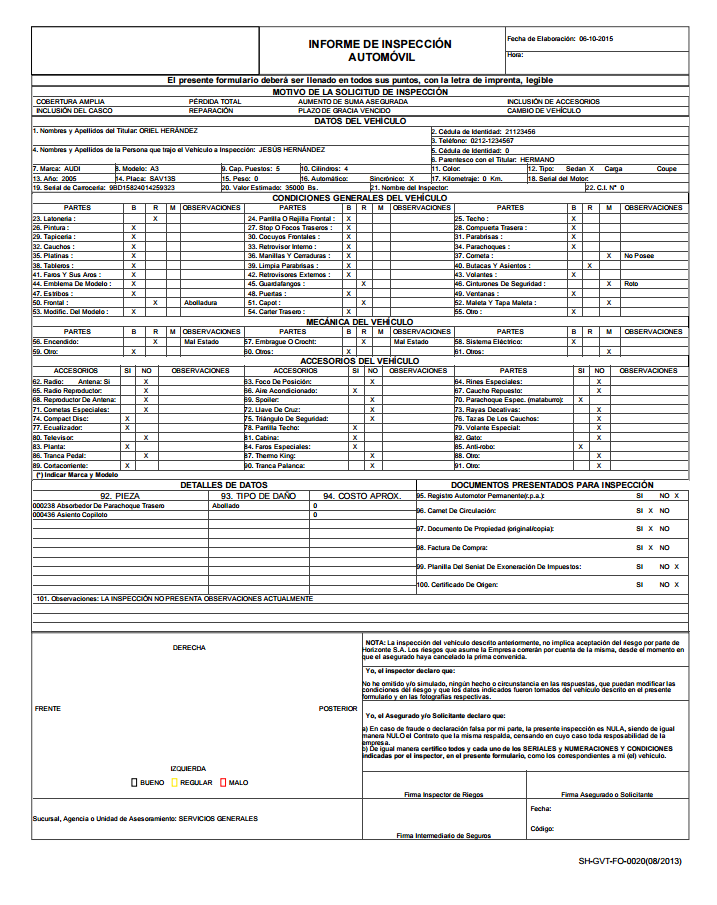
\includegraphics[width=\textwidth,height=18cm]{img/planilla_suscripcion.png}
\end{center}
\caption{Proceso de Suscripción. (2016)}
\label{fig:planilla_suscripcion}
\end{figure}
\setlength{\parskip}{0mm}
\chapter{Marco Metodológico}


\section{Metodología Tradicional} 
%%%%%%%%%%%%%%%%%%%%%%%%%%%%%%% RUP %%%%%%%%%%%%%%%%%%%%%%%%%%%%%%%%%%%
\subsection{RUP}

 RUP es un proceso para el desarrollo de un proyecto de software que define claramente quien, cómo, cuándo y qué debe hacerse en el proyecto, con 3 características esenciales, está dirigido por:

\begin{itemize}

    \item Los Casos de Uso : que orientan el proyecto a la importancia para el usuario y lo que este quiere. 

    \item La arquitectura: que Relaciona la toma de decisiones que indican cómo tiene que ser construido el sistema y en qué orden.

    \item Iterativo e incremental: dividiéndose el proyecto en mini proyectos donde los casos de uso y la arquitectura cumplen sus objetivos de manera más depurada.

\end{itemize}


\subsubsection{Ciclo de vida}
    RUP divide el proceso en 4 fases, dentro de las cuales se realizan varias iteraciones en número variable según el proyecto y en las que se hace un mayor o menor hincapié en los distintas actividades


\begin{figure}[H]
\begin{center}
	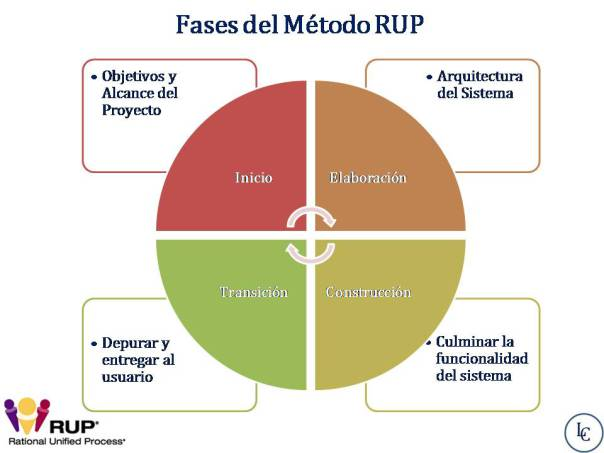
\includegraphics[width=13cm,height=8cm]{img/fases-rup.jpg}
\end{center}
\caption{Proceso RUP. (Tomada de \citet{dtyocbib} , 2016)}
\label{fig:Rup}
\end{figure}
%https://dtyoc.com/tag/johana-vincze/



\begin{itemize}

    \item Fase de Inicio: Esta fase tiene como propósito definir y acordar el alcance del proyecto con los patrocinadores, identificar los riesgos asociados al proyecto, proponer una visión muy general de la arquitectura de software y producir el plan de las fases y el de iteraciones posteriores.

	\item Fase de elaboración: En la fase de elaboración se seleccionan los casos de uso que permiten definir la arquitectura base del sistema y se desarrollaran en esta fase, se realiza la especificación de los casos de uso seleccionados y el primer análisis del dominio del problema, se diseña la solución preliminar.

	\item Fase de Desarrollo: El propósito de esta fase es completar la funcionalidad del sistema, para ello se deben clarificar los requisitos pendientes, administrar los cambios de acuerdo a las evaluaciones realizados por los usuarios y se realizan las mejoras para el proyecto.

	\item Fase de Transición: El propósito de esta fase es asegurar que el software esté disponible para los usuarios finales, ajustar los errores y defectos encontrados en las pruebas de aceptación, capacitar a los usuarios y proveer el soporte técnico necesario. Se debe verificar que el producto cumpla con las especificaciones entregadas por las personas involucradas en el proyecto.	

\end{itemize}

%https://es.scribd.com/doc/7844685/CONCEPTOS-DE-RUP
%%%%%%%%%%%%%%%%%%%%%%%%%%%%%%% END RUP %%%%%%%%%%%%%%%%%%%%%%%%%%%%%%%%%%%

%%%%%%%%%%%%%%%%%%%%%%%%%%%%%%% Cascada %%%%%%%%%%%%%%%%%%%%%%%%%%%%%%%%%%%
\pagebreak
\subsection{Cascada}

Modelo en Cascada, también llamado Lineal secuencial, es el enfoque metodológico que ordena rigurosamente las etapas del proceso para el desarrollo de software, de tal forma que el inicio de cada etapa debe esperar a la finalización de la etapa anterior. 

\subsubsection{Fases del Modelo}

\begin{figure}[H]
\begin{center}
	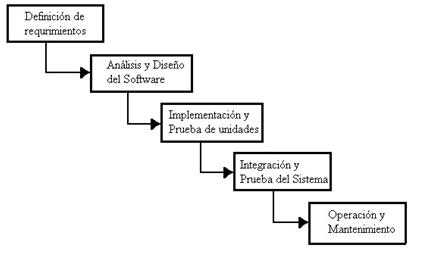
\includegraphics[width=13cm,height=8cm]{img/cascada.jpg}
\end{center}
\caption{Proceso Cascada. (Tomada de \citet{cascadabib}, 2013)}
\label{fig:Casacada}
\end{figure}

\begin{itemize}

    \item Análisis de requisitos: En esta fase se analizan las necesidades de los usuarios finales del software para determinar qué objetivos debe cubrir. De esta fase surge una memoria llamada SRD (documento de especificación de requisitos), que contiene la especificación completa de lo que debe hacer el sistema sin entrar en detalles internos. 

    %Es importante señalar que en esta etapa se debe consensuar todo lo que se requiere del sistema y será aquello 
    %lo que seguirá en las siguientes etapas, no pudiéndose requerir nuevos resultados a mitad del proceso de 
    %elaboración del software.

    \item Diseño del Sistema: Se descompone y organiza el sistema en elementos que puedan elaborarse por separado, aprovechando las ventajas del desarrollo en equipo. Como resultado surge el SDD (Documento de Diseño del Software), que contiene la descripción de la estructura relacional global del sistema y la especificación de lo que debe hacer cada una de sus partes, así como la manera en que se combinan unas con otras. 

    \item Diseño del Programa: Es la fase en donde se realizan los algoritmos necesarios para el cumplimiento de los requerimientos del usuario así como también los análisis necesarios para saber que herramientas usar en la etapa de Codificación.

    \item Codificación: Es la fase en donde se implementa el código fuente, haciendo uso de prototipos así como de pruebas y ensayos para corregir errores. Dependiendo del lenguaje de programación y su versión se crean las bibliotecas y componentes reutilizables dentro del mismo proyecto para hacer que la programación sea un proceso mucho más rápido.

    \item Pruebas: Los elementos, ya programados, se ensamblan para componer el sistema y se comprueba que funciona correctamente y que cumple con los requisitos, antes de ser entregado al usuario final.

    %Existen varios tipos de Pruebas:  Pruebas de unidad Pruebas de integración Pruebas de sistema Pruebas de %aceptación

    \item Verificación: Es la fase en donde el usuario final ejecuta el sistema, para ello el o los programadores ya realizaron exhaustivas pruebas para comprobar que el sistema no falle.

    \item Mantenimiento: Una de las etapas mas criticas, ya que se destina un 75 de los recursos, es el mantenimiento del Software ya que al utilizarlo como usuario final puede ser que no cumpla con todas nuestras expectativas.

    %Tipos de Mantenimiento: Preventivo y Perfectivo, Correctivo, Evolutivo

\end{itemize}

%http://www.ecured.cu/Modelo_en_cascada


%%%%%%%%%%%%%%%%%%%%%%%%%%%%%%% End Cascada %%%%%%%%%%%%%%%%%%%%%%%%%%%%%%%%%%%

\subsection{Cuadro Comparativo}

\begin{table}[H]	
\begin{center}
\begin{tabular}{ | m{6cm} | m{6cm} | } 
  \hline
 RUP & Casacada \\
 \hline
 Es un proceso iterativo.  & Es un proceso secuencial.  \\
 \hline
 Desarrolla el producto en base al feedback de los accionistas.  &   El proceso de creación del software tarda mucho tiempo ya que debe pasar por el proceso de prueba. \\
 \hline
  Cada iteracion produce una versión ejecutable. & Hasta que el software no esté completo no se opera. Esto es la base para que funcione bien. \\
 \hline
  Es un marco adaptable de procesos de software & Es un proceso concreto definido. \\
 \hline
\end{tabular}
\caption{Tabla comparativa de metodologías tradicionales}
\label{Tabla:1}
\end{center}
\end{table}	
.


\section{Metodología Ágil} 

El desarrollo ágil de software envuelve un enfoque para la toma de decisiones en los proyectos basados en el desarrollo iterativo e incremental, donde los requisitos y soluciones evolucionan con el tiempo según la necesidad del proyecto. Así el trabajo es realizado mediante la colaboración de equipos auto-organizados y multidisciplinarios, inmersos en un proceso compartido de toma de decisiones a corto plazo.

%%%%%%%%%%%%%%%%%%%%%%%%%%%%%%% Scrum %%%%%%%%%%%%%%%%%%%%%%%%%%%%%%%%%%%

\subsection{SCRUM}
\setlength{\parskip}{5mm}
El Scrum es un proceso de la Metodología Ágil que se usa para minimizar los riesgos durante la realización de un proyecto, pero de manera colaborativa. 

Entre las ventajas se encuentran la productividad, calidad y que se realiza un seguimiento diario de los avances del proyecto, logrando que los integrantes estén unidos, comunicados y que el cliente vaya viendo los avances.
\setlength{\parskip}{0mm}
\subsubsection{Ciclo de vida}


\begin{figure}[H]
\begin{center}
	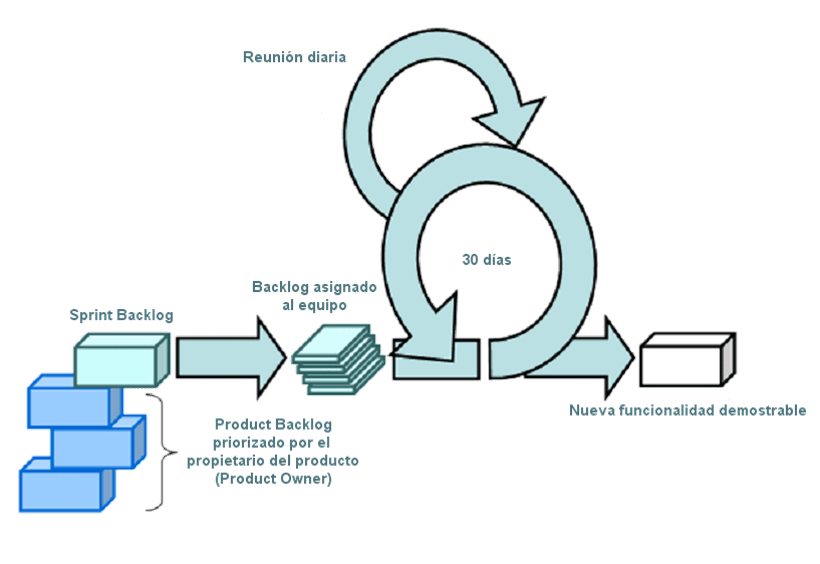
\includegraphics[width=13cm,height=8cm]{img/scrum.png}
\end{center}
\caption{Proceso Scrum. (Tomada de \citet{scrumibib}, 2004)}
\label{fig:Scrum}
\end{figure}

\subsubsection{Spring}
\setlength{\parskip}{5mm}

	Es el periodo de tiempo durante el que se desarrolla un incremento de funcionalidad dura máximo 30 días. Constituye el núcleo de Scrum, que divide de esta forma el desarrollo de un proyecto en un conjunto de pequeñas “carreras”. Durante el proceso no se puede modificar el trabajo que se ha acordado en el Backlog, solo es posible cambiar el curso de un sprint abortándolo y esto solo puede hacerlo el Scrum Master. 
	
\setlength{\parskip}{0mm}

\subsubsection{Planificación del sprint}
\setlength{\parskip}{5mm}

	En esta reunión se toman como base las prioridades y necesidades de negocio del cliente, y se determinan cuáles y cómo van a ser las funcionalidades que se incorporarán al producto en el siguiente sprint. Se trata de  una reunión conducida por  el responsable del funcionamiento  del marco scrum (Scrum Master en scrum técnico, o un miembro del equipo,en scrum pragmático) a la que deben asistir el propietario del producto y el equipo completo, y a la que también pueden asistir otros implicados en el proyecto.

	La reunión puede durar una jornada de trabajo completa, cuando se trata de planificar un sprint largo (de un mes de duración) o un tiempo proporcional para planificar un sprint más breve. Esta reunión debe dar respuesta a dos cuestiones:

	\begin{itemize}
		\item Qué se entregará al terminar el sprint.

		\item Cuál es el trabajo necesario para realizar el incremento previsto, y cómo lo llevará a cabo el equipo.
	\end{itemize}

\setlength{\parskip}{0mm}
	La  reunión  se  articula  en  dos  partes  de  igual  duración,  para  dar  respuesta  a  una  de  estas  cuestiones,en cada una.
	
\setlength{\parskip}{0mm}

\subsubsection{Scrum diario}
\setlength{\parskip}{5mm}

	Reunión diaria breve, de no más de 15 minutos, en la que el equipo sincroniza el trabajo y establece el plan para las 24 horas siguientes. Informa el avance de cada miembro del equipo e identifica posible necesidades e impedimentos.
	
\setlength{\parskip}{0mm}

\subsubsection{Revisión de las Iteraciones}
\setlength{\parskip}{5mm}

	Al finalizar cada sprint se revisa funcionalmente el resultado, con todos los implicados en el proyecto. Es por tanto la duración del sprint, el período de tiempo máximo para descubrir planteamientos erróneos, mejorables o mal interpretaciones en las funcionalidades del producto.
	
\setlength{\parskip}{0mm}


\subsubsection{Retrospectiva}
\setlength{\parskip}{5mm}

	Reunión que se realiza tras la revisión de cada sprint, y antes de la reunión de planificación del siguiente, con una duración recomendada de una a tres horas, según la duración del sprint terminado.En ella el equipo realiza auto análisis de su sobre su forma de trabajar, e identifica fortalezas y  puntos débiles. El objetivo es consolidar y afianzar las primeras, y planificar acciones de mejora sobre los segundos.

	El objetivo de la revisión del sprint es analizar “QUÉ” se está construyendo, mientras que una reunión retrospectiva se centra en “CÓMO” lo estamos construyendo: “CÓMO” estamos trabajando, con el objetivo de analizar problemas y aspectos mejorables.

	Las reuniones "retrospectivas" realizadas de forma periódica por el equipo para mejorar la forma de trabajo, se consideran cada vez más un componente del marco técnico de scrum, si bien no es una reunión para seguimiento de la evolución del producto, sino para mejora del marco de trabajo.(Juan Palacio,2014)
\setlength{\parskip}{0mm}

%http://www.scrummanager.net/files/sm_proyecto.pdf
%%%%%%%%%%%%%%%%%%%%%%%%%%%%%%% END Scrum %%%%%%%%%%%%%%%%%%%%%%%%%%%%%%%%%%%
    

%%%%%%%%%%%%%%%%%%%%%%%%%%%%%%% XP %%%%%%%%%%%%%%%%%%%%%%%%%%%%%%%%%%%
\subsection{XP}
\setlength{\parskip}{5mm}
Es una metodología ágil centrada en potenciar las relaciones interpersonales como clave para el éxito en desarrollo de software, promoviendo el trabajo en equipo, preocupándose por el aprendizaje de los desarrolladores, y propiciando un buen clima de trabajo. XP se basa en realimentación continua entre el cliente y el equipo de desarrollo, comunicación fluida entre todos los participantes, simplicidad en las soluciones implementadas y coraje para enfrentar los cambios. XP se define como especialmente adecuada para proyectos con requisitos imprecisos, muy cambiantes, y donde existe un alto riesgo técnico.
\setlength{\parskip}{0mm}
% \subsubsection{Prácticas básicas de la programación extrema}
% \setlength{\parskip}{5mm}

% \begin{itemize}

%     \item Equipo completo: Forman parte del equipo todas las personas que tienen algo que ver con el proyecto, incluido el cliente y el responsable del proyecto. 

% 	\item Planificación: Se hacen las historias de usuario y se planifica en qué orden se van a hacer y las mini-versiones. La planificación se revisa continuamente. 
	
% 	\item Test del cliente: El cliente, con la ayuda de los desarrolladores, propone sus propias pruebas para validar las mini-versiones. 

% 	\item Versiones pequeñas: Las mini-versiones deben ser lo suficientemente pequeñas como para poder hacer una cada pocas semanas. Deben ser versiones que ofrezcan algo útil al usuario final y no trozos de código que no pueda ver funcionando. 

% 	\item Diseño simple: Hacer siempre lo mínimo imprescindible de la forma más sencilla posible. Mantener siempre sencillo el código. 

% 	\item Pareja de programadores: Los programadores trabajan por parejas (dos delante del mismo ordenador) y se intercambian las parejas con frecuencia (un cambio diario). 

% 	\item Desarrollo guiado por las pruebas automáticas: Se deben realizar programas de prueba automática y deben ejecutarse con mucha frecuencia. Cuantas más pruebas se hagan, mejor. 

% 	\item Integración continua: Deben tenerse siempre un ejecutable del proyecto que funcione y en cuanto se tenga una nueva pequeña funcionalidad, debe recompilarse y probarse. Es un error mantener una versión congelada dos meses mientras se hacen mejoras y luego integrarlas todas de golpe. Cuando falle algo, no se sabe qué es lo que falla de todo lo que hemos metido. 

% 	\item El código es de todos: Cualquiera puede y debe tocar y conocer cualquier parte del código. Para eso se hacen las pruebas automáticas. 

% 	\item Normas de codificación: Debe haber un estilo común de codificación (no importa cual), de forma que parezca que ha sido realizado por una única persona. 

% 	\item Metáforas: Hay que buscar unas frases o nombres que definan cómo funcionan las distintas partes del programa, de forma que sólo con los nombres se pueda uno hacer una idea de qué es lo que hace cada parte del programa. Un ejemplo claro es el "recolector de basura" de java. Ayuda a que todos los programadores (y el cliente) sepan de qué estamos hablando y que no haya mal entendidos. 

% 	\item Ritmo sostenible: Se debe trabajar a un ritmo que se pueda mantener indefinidamente. Esto quiere decir que no debe haber días muertos en que no se sabe qué hacer y que no se deben hacer un exceso de horas otros días. Al tener claro semana a semana lo que debe hacerse, hay que trabajar duro en ello para conseguir el objetivo cercano de terminar una historia de usuario o mini-versión. 


% \end{itemize}
% \setlength{\parskip}{0mm}
\subsubsection{Ciclo de vida}

\setlength{\parskip}{5mm}
Un proyecto XP tiene éxito cuando el cliente selecciona el valor de negocio a implementar basado en la habilidad del equipo para medir la funcionalidad que puede entregar a través del tiempo. El ciclo de desarrollo consiste (a grandes rasgos) en los siguientes pasos:

\begin{itemize}

	\item El cliente define el valor de negocio a implementar.

	\item El programador estima el esfuerzo necesario para su implementación.

	\item El cliente selecciona qué construir, de acuerdo con sus prioridades y las restricciones de tiempo.

	\item El programador construye ese valor de negocio.

	\item Vuelve al paso 1.

\end{itemize}
    
En todas las iteraciones de este ciclo tanto el cliente como el programador aprenden. No se debe presionar al programador a realizar más trabajo que el estimado, ya que se perderá calidad en el software o no se cumplirán los plazos. De la misma forma el cliente tiene la obligación de manejar el ámbito de entrega del producto, para asegurarse que el sistema tenga el mayor valor de negocio posible con cada iteración.

El ciclo de vida ideal de XP consiste de seis fases: % Exploración, Planificación de la Entrega (Release), Iteraciones, Producción, Mantenimiento y Muerte del Proyecto.
\setlength{\parskip}{0mm}

\begin{figure}[H]
\begin{center}
	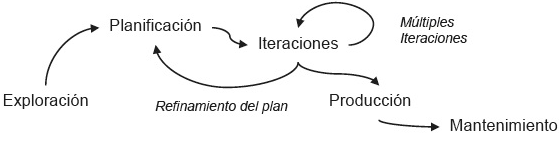
\includegraphics[width=\textwidth,height=5cm]{img/xp.png}
\end{center}
\caption{Proceso Scrum. (Tomada de \citet{xpibib}, 2004)}
\label{fig:xp}
\end{figure}

\subsubsection{Fase I: Exploración}	
\setlength{\parskip}{5mm}

	En esta fase, los clientes plantean a grandes rasgos las historias de usuario que son de interés para la primera entrega del producto. Al mismo tiempo el equipo de desarrollo se familiariza con las herramientas, tecnologías y prácticas que se utilizarán en el proyecto. Se prueba la tecnología y se exploran las posibilidades de la arquitectura del sistema construyendo un prototipo. La fase de exploración toma de pocas semanas a pocos meses, dependiendo del tamaño y familiaridad que tengan los programadores con la tecnología.

\setlength{\parskip}{0mm}

\subsubsection{Fase II: Planificación de la Entrega}
\setlength{\parskip}{5mm}

	En esta fase el cliente establece la prioridad de cada historia de usuario, y correspondientemente, los programadores realizan una estimación del esfuerzo necesario de cada una de ellas. Se toman acuerdos sobre el contenido de la primera entrega y se determina un cronograma en conjunto con el cliente. Una entrega debería obtenerse en no más de tres meses. Esta fase dura unos pocos días.

	Las estimaciones de esfuerzo asociado a la implementación de las historias la establecen los programadores utilizando como medida el punto. Un punto, equivale a una semana ideal de programación. Las historias generalmente valen de 1 a 3 puntos. Por otra parte, el equipo de desarrollo mantiene un registro de la "velocidad" de desarrollo, establecida en puntos por iteración, basándose principalmente en la suma de puntos correspondientes a las historias de usuario que fueron terminadas en la última iteración.

	La planificación se puede realizar basándose en el tiempo o el alcance. La velocidad del proyecto es utilizada para establecer cuántas historias se pueden implementar antes de una fecha determinada o cuánto tiempo tomará implementar un conjunto de historias. Al planificar por tiempo, se multiplica el número de iteraciones por la velocidad del proyecto, determinándose cuántos puntos se pueden completar. Al planificar según alcance del sistema, se divide la suma de puntos de las historias de usuario seleccionadas entre la velocidad del proyecto, obteniendo el número de iteraciones necesarias para su implementación.	

\setlength{\parskip}{0mm}

\subsubsection{Fase III: Iteraciones}
\setlength{\parskip}{5mm}

	Esta fase incluye varias iteraciones sobre el sistema antes de ser entregado. El Plan de Entrega está compuesto por iteraciones de no más de tres semanas. En la primera iteración se puede intentar establecer una arquitectura del sistema que pueda ser utilizada durante el resto del proyecto. Esto se logra escogiendo las historias que fuercen la creación de esta arquitectura, sin embargo, esto no siempre es posible ya que es el cliente quien decide qué historias se implementarán en cada iteración (para maximizar el valor de negocio). Al final de la última iteración el sistema estará listo para entrar en producción.

	Los elementos que deben tomarse en cuenta durante la elaboración del Plan de la Iteración son: historias de usuario no abordadas, velocidad del proyecto, pruebas de aceptación no superadas en la iteración anterior y tareas no terminadas en la iteración anterior. Todo el trabajo de la iteración es expresado en tareas de programación, cada una de ellas es asignada a un programador como responsable, pero llevadas a cabo por parejas de programadores. Wake en proporciona algunas guías útiles para realizar la planificación de la entrega y de cada iteración.


\setlength{\parskip}{0mm}

\subsubsection{Fase IV: Producción}
\setlength{\parskip}{5mm}

	La fase de producción requiere de pruebas adicionales y revisiones de rendimiento antes de que el sistema sea trasladado al entorno del cliente. Al mismo tiempo, se deben tomar decisiones sobre la inclusión de nuevas características a la versión actual, debido a cambios durante esta fase.

	Es posible que se rebaje el tiempo que toma cada iteración, de tres a una semana. Las ideas que han sido propuestas y las sugerencias son documentadas para su posterior implementación (por ejemplo, durante la fase de mantenimiento).

\setlength{\parskip}{0mm}

\subsubsection{Fase V: Mantenimiento}
\setlength{\parskip}{5mm}

	Mientras la primera versión se encuentra en producción, el proyecto XP debe mantener el sistema en funcionamiento al mismo tiempo que desarrolla nuevas iteraciones. Para realizar esto se requiere de tareas de soporte para el cliente. De esta forma, la velocidad de desarrollo puede bajar después de la puesta del sistema en producción. La fase de mantenimiento puede requerir nuevo personal dentro del equipo y cambios en su estructura.

\setlength{\parskip}{0mm}

\subsubsection{Fase VI: Muerte del Proyecto}
\setlength{\parskip}{5mm}

	Es cuando el cliente no tiene más historias para ser incluidas en el sistema. Esto requiere que se satisfagan las necesidades del cliente en otros aspectos como rendimiento y confiabilidad del sistema. Se genera la documentación final del sistema y no se realizan más cambios en la arquitectura. La muerte del proyecto también ocurre cuando el sistema no genera los beneficios esperados por el cliente o cuando no hay presupuesto para mantenerlo.

\setlength{\parskip}{0mm}

% http://ingenieriadesoftware.mex.tl/images/18149/PROGRAMACI%C3%93N%20EXTREMA.pdf
%%%%%%%%%%%%%%%%%%%%%%%%%%%%%%% END XP %%%%%%%%%%%%%%%%%%%%%%%%%%%%%%%%%%%

%%%%%%%%%%%%%%%%%%%%%%%%%%%%%%% Agilus %%%%%%%%%%%%%%%%%%%%%%%%%%%%%%%%%%%

\subsection{Agilus}
\setlength{\parskip}{5mm}

	El Método AgilUs es un método de desarrollo ágil, resultado de una de las líneas de investigación desarrolladas en el Centro de Ingeniería de Software y Sistemas (ISYS) de la Escuela de Computación, Universidad Central de Venezuela. Se basa en el concepto de usabilidad, en la necesidad de desarrollar software usables. Se fundamenta en el análisis centrado en el usuario y en la participación de especialistas, con el objetivo de evolucionar el software, a fin de que éste alcance el mayor grado de usabilidad una vez culminado su desarrollo.
	
	AgilUs es un método de desarrollo iterativo e incremental que pone el mayor peso del desarrollo en la consecución de la usabilidad. Se centra en que la construcción y desarrollo de las interfaces de usuario no debe ser una adición estética que se da al final del desarrollo del sistema sino, muy por el contrario, el desarrollo de interfaces de usuario debe guiar las decisiones en Ingeniería de Software. En AgilUs son los usuarios, y no el cliente ni los programadores quienes guían el desarrollo del proyecto.

	El Método AgilUs busca proporcionar un conjunto de actividades organizadas para construir la usabilidad en el diseño de interfaces de usuario durante el desarrollo de un producto de software. El proceso de desarrollo de software engloba las actividades de requisitos, análisis, prototipaje y entrega; así como las evaluaciones de usabilidad correspondientes a cada etapa del proceso. Se realizan en ciclos iterativos hasta alcanzar el producto final. En cada etapa del proceso de desarrollo de software, se incluyen actividades propias para la construcción de la usabilidad.

\setlength{\parskip}{0mm}

\subsubsection{Ciclo de vida}
\setlength{\parskip}{5mm}
	El ciclo de vida de AgilUs hace énfasis en la importancia del usuario y sus evaluaciones. Está basado en el desarrollo iterativo e incremental de prototipos de alta fidelidad hasta que se convierten en el producto final para entrega. Este producto final puede ser posteriormente modificado a través de un mantenimiento correctivo y/o evolutivo, que no está contemplado como parte del método.
	\setlength{\parskip}{0mm}

\begin{figure}[H]
\begin{center}
	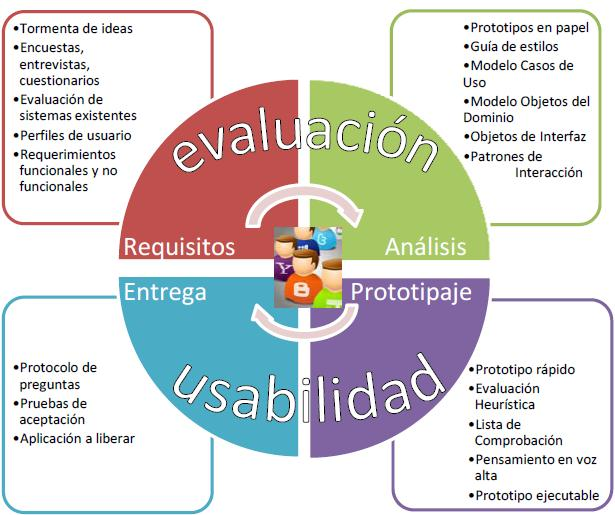
\includegraphics[width=13cm,height=8cm]{img/agilus.jpg}
\end{center}
\caption{El método AgilUs: etapas, actividades y artefactos.}
\label{fig:Agilus}
\end{figure}
%https://dtyoc.com/tag/johana-vincze/



\begin{itemize}

    \item Requisitos: Se realiza el análisis global del problema a solucionar, se estudian productos similares existes, se genera un perfil de usuario, y se define la lista de requerimientos a desarrollar. Esta etapa es importante en el desarrollo del software, ya que un mal análisis de requisitos traería como consecuencia un software que no cumple con las necesidades del usuario.

    \item Análisis: Se lleva a cabo el análisis de la solución a desarrollar, se emplean diagramas de casos de uso y modelo de objetos del dominio, siguiendo la notación UML, para definir las funcionalidades que tendrá el producto a desarrollar.

    \item Prototipaje: Se implementa un prototipo rápido de la interfaz de usuario a partir de los patrones de interacción, el cual va evolucionando hasta convertirse en el producto final, se genera la guía de estilo, y se realizan evaluaciones de usabilidad apropiadas a esta etapa: las evaluaciones heurísticas y las listas de comprobación.

    \item Entrega: Se aplican las pruebas al sistema para certificar que la aplicación desarrollada sea un software usable y sin errores, finalmente se pone en producción la aplicación.

\end{itemize}

(\citet{agilusbib}, 2011) 
\newpage
\subsection{Cuadro Comparativo}


\begin{table}[H]	
\begin{center}
\begin{tabular}{ | m{4cm} | m{4cm}| m{4cm}| } 
 \hline
 Scrum & XP & Agilus \\
 \hline
 Las iteraciones de entrega son de dos a cuatro semanas y se conocen como sprint. 
 &
 Las iteraciones de entrega son de una a tres semanas (algo más rápidas). 
 & 
 Las iteraciones de entrega son de una a dos semanas aproximadamente.\\
 \hline
 Al finalizar un sprint, las tareas que se han realizado del Sprint Backlog y en las que el Product Owner ha mostrado su conformidad ya no se vuelven a tocar en ningún momento. "Lo que se terminar, funciona y está bien, se aparta y ya no se toca".
 & 
 Las tareas que se van terminando en las diferentes entregas al cliente son susceptibles a modificaciones durante el transcurso de todo el proyecto, incluso después de que funcionen correctamente.
 & 
 El equipo de desarrollo produce un primer prototipo y a partir de las observaciones, retroalimentación se produce el siguiente.\\
 \hline
 El scrum team trata de seguir el orden de prioridad que marca el Product Owner en el Sprint Backog pero si ven que es mejor modificar el orden de prioridad para el desarrollo de tareas, pueden hacerlo.
 & 
 El equipo de desarrollo sigue estrictamente el orden de prioridad de las tareas definido por el cliente (aunque el equipo de desarrollo le ayude a decidir, ellos son los que mandan).
 & 
 El equipo de desarrollo sigue estrictamente el orden de prioridad definido para cada una de las fases.\\
 \hline
 El Scrum es una metodología de desarrollo ágil más basada en la administración del proyecto.
 & 
 En cambio, el XP se centra más en la propia programación o creación del producto.
 & 
 Agilus en cambio se centra más el desarrollo en la usabilidad del producto de software.\\
 \hline
 Cada miembro del "Scrum Team" trabaja de forma individual.
 & 
 Los miembros programa en parejas en un proyecto de XP.
 & 
 Los miembros del equipo trabajan en conjunto para completar cada fase de desarrollo.\\
 \hline
 % El Scrum se originó en 1986 tiene una estructura más jerárquica y es más utilizado.
 % & 
 % El XP en cambio, no se desarrolló hasta finales de los noventa.
 % & 
 % .\\
 % \hline
\end{tabular}
\caption{Tabla comparativa de metodologías ágiles}
\label{Tabla:2}
\end{center}
\end{table}	







\section{Cuadro comparativo [Metodologías Tradicionales vs Ágiles]} 

%%%%%%%%%%%%%%%%%%%%%%%%%%%%%%% END Agilus %%%%%%%%%%%%%%%%%%%%%%%%%%%%%%%%%%%
\begin{table}[H]	
\begin{center}
\begin{tabular}{ | m{6cm} | m{6cm} | } 
 \hline
 Tradicionales & Ágiles \\ 
	\hline
	Basadas en normas provenientes de estándares seguidos por el entorno de desarrollo.  Posee cierta resistencia a los cambios. 
	&
	Basadas en heurísticas provenientes de prácticas de producción de código las cuales previenen cambios durante el proyecto.\\ 
 	\hline
 	Define un proceso mucho más controlado junto con numerosas políticas/normas.
	&
	Define un proceso menos controlado, con pocos principios.\\ 
	\hline
	El cliente interactúa con el equipo de desarrollo mediante reuniones.	
	&
	El cliente es parte del equipo de desarrollo. \\ 
	\hline
	Genera más artefactos.	
	&
	Genera pocos artefactos.\\ 
	\hline

	Más roles.	
	&
	Pocos roles.\\ 
	\hline

	Grupos grandes y posiblemente distribuidos.	
	&
	Grupos pequeños (<10 integrantes) y trabajando en el mismo sitio.\\ 
	\hline

	Dependencia de la arquitectura de software mediante modelos.	
	& 
	Menor dependencia de la arquitectura de software.\\ 
	\hline

	Existe un contrato prefijado.	
	&
	No existe contrato tradicional o al menos es bastante flexible.\\ 
	\hline

\end{tabular}
\caption{Diferencias entre metodologías ágiles y tradicionales}
\label{Tabla:3}
\end{center}
\end{table}	

%https://es.scribd.com/doc/91676941/Metodologias-agiles-vs-tradicionales
%http://rdsoporteymantenimientodepc.blogspot.com/2014/03/metodologias-de-desarrollo-agiles-vs.html

%https://es.scribd.com/doc/36570454/Diferencia-Entre-PostgreSQL-MySQL-Oracle
\chapter{Marco Aplicativo}


\section{Descripción general de la solución} 
\setlength{\parskip}{5mm}
\setlength{\parskip}{0mm}


\section{Aplicación de la metodología Scrum}

\subsection{Lista de Objetivos (Pila del Producto)}



\begin{table}[htb]	
\begin{center}
\begin{tabular}{ | m{2cm} | m{9cm}| m{3cm}| } 
 \hline
 Sprint & Actividad & Fecha \\
 \hline
 1. 
 & 
 \begin{itemize}
 	\item Instalación de las herramientas de desarrollo necesarias.
 	\item Configuración de los ambientes de desarrollo.
 	\item Maquetado de las Interfaces
 	\item Elaboración del Diagrama de Modelo relacional para la base de datos.
 \end{itemize}
 & 
 01/02/2017 - 14/02/2017\\
 \hline

 2. 
 & 
 \begin{itemize}
 	\item Desarrollo del modulo de registro.
 	\item Realización de pruebas de funcionalidad.
 \end{itemize}
 & 
 15/02/2017 - 28/02/2017\\
 \hline

 3.
 & 
 \begin{itemize}
 	\item Desarrollo de la funcionalidad de recuperar contraseña
 	\item Desarrollo del modulo de gestión de solicitudes
 	\item Desarrollo de la funcionalidad de solicitar inspección
 	\item Realización de pruebas de funcionalidad
 \end{itemize}
 & 
 01/03/2017 - 15/03/2017\\
 \hline
 
 4.
 & 
 \begin{itemize}
 	\item Desarrollo de la funcionalidad de gestión de tickets de solicitudes de inspección
 	\item Desarrollo de la funcionalidad de consultar solicitudes de inspección
 	\item Realización de pruebas de funcionalidad
 \end{itemize}
 & 
 16/03/2017 - 31/03/2017\\
 \hline
 
 5. 
 & 
 \begin{itemize}
 	\item Desarrollo de la funcionalidad de realizar inspección
 	\item Desarrollo de la funcionalidad de gestionar inspección
 	\item Desarrollo de la funcionalidad de generación de pdf
 	\item Realización de pruebas de funcionalidad
 \end{itemize}
 & 
 01/04/2017 - 15/04/2017\\
 \hline

 6. 
 & 
 \begin{itemize}
 	\item Desarrollo del modulo administrativo
 	\item Desarrollo de la funcionalidad de Gestión de Usuarios (Taquilla Inspectores)
 	\item Realización de pruebas de funcionalidad
 \end{itemize}
 & 
 16/04/2017 - 30/04/2017\\
 \hline

 7. 
 & 
 \begin{itemize}
 	\item Desarrollo de la funcionalidad de Gestión de Titulares de Vehículo
 	\item Desarrollo de la funcionalidad de Gestión de Personas que trajeron el Vehículo a la inspección
 	\item Realización de pruebas de funcionalidad
 \end{itemize}
 & 
 01/05/2017 - 15/05/2017\\
 \hline

 8.
 & 
 \begin{itemize}
 	\item Desarrollo del Vehículo en formato SVG
 	\item Realización de pruebas de funcionalidad
 \end{itemize}
 &
 16/05/2017 - 30/05/2017\\
 \hline

\end{tabular}
\caption{Pila del Producto}
\label{Tabla:15}
\end{center}
\end{table}	



\subsection{Lista de tareas de la iteración (Pila del Sprint)}
\setlength{\parskip}{5mm}

\textbf{-Sprint 1}: Se comenzó con la instalación de las herramientas necesarias para el desarrollo de la aplicación, las cuales fueron Python 2.7.9, PostgreSQL 9.4.3 y Django 1.10. 

Además se realizó el diseño y maquetado de la aplicación, a partir de los componente provistos por el Framework Bootstrap 4 y HMTL5 como base para el desarrollo de las interfaces de usuario. También se realizo el modelado de la base de datos en conjunto con los diagramas asociados al sistema. Finalmente se instalaron todas las dependencias necesarias en un ambiente virtual para la realización del sistema.


\textbf{-Sprint 2}: En este Sprint se desarrollaron parte de las funcionalidades pertinentes al modulo de registro, con sus validaciones respectivas para el correcto funcionamiento del sistema de registro. Luego se realización las pruebas de funcionalidad correspondientes para validar el funcionamiento esperado del sistema.

\textbf{-Sprint 3}: En este Sprint se terminaron de desarrollar las funcionalidades restantes del modulo de registro, se empezó el desarrollo del modulo de gestión de solicitudes, en el cual se implementaron parte de las funcionalidades tales como el solicitar una inspección. Además se realizaron las pruebas pertinentes para el correcto funcionamiento de la aplicación.

\textbf{-Sprint 4}: Se realizaron las funcionalidades de gestión de tickets de solicitud de inspección y consultar solicitudes de inspección, en esta ultima se obtuvieron las especificaciones de los campos por los cuales se filtrarían dichas solicitudes. Luego se realizaron las pruebas necesarias para validar el correcto funcionamiento de las funcionalidades desarrolladas.

\textbf{-Sprint 5}: En este Sprint se desarrollaron las funcionalidades de realizar inspección y la gestión de las mismas, además de la generación de la planilla en la cual se registran todos los datos de las especificaciones del vehículo e información relevante de la inspección. Se realizaron las pruebas funcionales para validar el correcto funcionamiento.

\textbf{-Sprint 6}: En este Sprint se desarrollo parte del modulo de administración, en especifico la funcionalidad de gestión de usuarios que comprende en editar, inactiva y eliminar usuarios. Además se realizaron las pruebas pertinentes para garantizar la correcta funcionalidad.

\textbf{-Sprint 7}: Se desarrollaron las funcionalidades restantes del modulo de administración, gestión de los titulares del vehículo y de las personas que trajeron el vehículo a inspeccionar. Seguidamente se realizaron las pruebas funcionales para validar un correcto funcionamiento.

\textbf{-Sprint 8}: Se desarrollo la imagen del carro en formato SVG y se validaron las partes pertinente para que cambiaran de color dependiendo del estado del vehículo. Se realizaron las pruebas correspondientes para finalizar la planilla de inspección.

\setlength{\parskip}{0mm}


\section{Requerimientos del Sistema } 
\setlength{\parskip}{5mm}
	De acuerdo a los requerimientos definidos por el cliente (Product Owner), se estableció las siguiente clasificación:

	\textbf{-Requerimientos Funcionales}: 

	\begin{itemize}
		\item Registro de usuarios por roles.
		\item Recuperar contraseña.
		\item Edición del perfil de usuario.
		\item Administración de los usuarios del sistema.
		\item Administración de los clientes del sistema (Titular, Persona que trajo el Vehículo).
		\item Creación de tickets para la inspección del vehículo.
		\item Consultar tickets creados.
		\item Consultar solicitudes de inspección.
		\item Registro de los datos de la inspección del vehículo.
		\item Gestionar solicitudes de inspección.
		\item Creación de una imagen de carro donde se muestren diferentes colores, para las partes del carro, dependiendo su estado.
	\end{itemize}

	\textbf{-Requerimientos no Funcionales}: 

	\begin{itemize}
		\item Validar las entradas de los datos para el correcto funcionamiento del sistema.
	\end{itemize}

\setlength{\parskip}{0mm}


\section{Perfiles de Usuario} 
\setlength{\parskip}{5mm}

\textbf{-Administrador}: Es el usuario encargado de gestionar tanto usuarios como a los clientes y propietarios de los vehículos inspeccionados.
	\begin{itemize}
		\item Búsqueda de usuarios del sistema.
		\item Búsqueda de titulares de los vehículos.
		\item Búsqueda de personas trajeron el vehículo a revisión. 
		\item Edición de titulares de vehículos.
		\item Edición de personas trajeron el vehículo a revisión.
		\item Edición y desactivación de usuarios Inspectores.
		\item Edición y desactivación de usuarios Taquilla.
		\item Reinicio de usuarios enviado les nuevas contraseñas.
	\end{itemize}

\textbf{-Inspector}: Este usuario puede crear una cuenta en el sistema para gestionar solicitudes de inspección de vehículo. También puede editar la información de su cuenta, ver la información de las solicitudes cerradas. 
	\begin{itemize}
		\item Creación y edición de una cuenta con su información básica para el uso del sistema.
		\item Visualización de las solicitudes de inspección pendientes por realizar.
		\item Vaciado de la información de la inspección del vehículo en el sistema.
		\item Gestión de la solicitud de inspección (verificación y guardado). 
		\item Visualizar información de las solicitudes de inspección.
		\item Búsqueda de solicitudes de inspección realizadas.
	\end{itemize}

\textbf{-Taquilla}: Este usuario puede crear una cuenta en el sistema para gestionar los tickets de atención, de las persona que requieran realizar una inspección.
	\begin{itemize}
		\item Creación y edición de una cuenta con su información básica para el uso del sistema.
		\item Creación de ticket para solicitud de inspección.
		\item Cancelar un ticket abierto de una solicitud de inspección 
		\item Búsqueda de tickets abiertos
	\end{itemize}


\setlength{\parskip}{0mm}


\section{Descripción del flujo asociado a la solución} 
\setlength{\parskip}{5mm}
\setlength{\parskip}{0mm}

\subsection{Proceso de creación de solicitud}
\setlength{\parskip}{5mm}
\setlength{\parskip}{0mm}

\subsection{Proceso de llenado de planilla de inspección}
\setlength{\parskip}{5mm}
\setlength{\parskip}{0mm}

\subsection{Proceso de gestión de solicitud de inspección}
\setlength{\parskip}{5mm}
\setlength{\parskip}{0mm}


\section{Análisis del modelo de datos y definición} 
\setlength{\parskip}{5mm}

En la elaboracion del modelo de datos pertenecientes a la aplicacion se crearon un total de veintiocho (28) tablas.

\setlength{\parskip}{0mm}

\subsection{Listado de tablas de la aplicación}

\setlength{\parskip}{5mm}

A continuación se presenta un listado con todas las tablas de la base de datos perteneciente al sistema desarrollado, junto con una breve descripción para cada una:


\textbf{-registro\_status}: Permite clasificar el estado del usuario (Activo,Inactivo).

\textbf{-registro\_tipousuario}: Permite clasificar a los usuarios por tipo (Administrador, Cliente, Taquilla).

\textbf{-registro\_usuario}: Permite almacenar los usuarios en el sistema.

\textbf{-rcs\_accesoriosbase}: Permite almacenar los accesorios básicos de la planilla.

\textbf{-rcs\_accesoriosvehiculo}: Tabla utilizada para representar los accesorios base de un vehículo.

\textbf{-rcs\_condicionesgeneralesbase}: Permite almacenar las condiciones generales básicas de la planilla.

\textbf{-rcs\_condicionesgeneralesvehiculo}: Tabla utilizada para representar las condiciones generales base de un vehículo.

\textbf{-rcs\_detallesdatos}: Permite almacenar lo detalles y datos de la planilla.

\textbf{-rcs\_documentospresentados}: Permite almacenar los documentos presentados básicos de la planilla.

\textbf{-rcs\_documentospresentadosbase}: Tabla utilizada para representar los documentos presentados base de un vehículo.

\textbf{-rcs\_estadosolicitud}: Permite almacenar los diferentes estado que puede poseer la planilla (Abierta, Por Revisar,Cerrada).

\textbf{-rcs\_estadovehiculo}: Permite almacenar los diferentes estado que puede poseer las partes del vehículo (Bueno, Regular,Malo).

\textbf{-rcs\_mecanicabase}: Permite almacenar las mecánicas básicas de la planilla.

\textbf{-rcs\_mecanicavehiculo}: Tabla utilizada para representar las mecánicas base de un vehículo.

\textbf{-rcs\_motivosolicitud}: Permite almacenar los diferentes motivos por lo cual se realiza la solicitud de inspección.

\textbf{-rcs\_solicitudinspeccion}: Permite almacenar las solicitudes de inspección realizadas por el sistema.

\textbf{-rcs\_tipomanejo}: Permite almacenar los diferentes tipos de manejo (Automático, Sincrónico).

\textbf{-rcs\_tipovehiculo}: Permite guardar la información de los diferentes tipos de vehículos (Sedan, Carga, Coupe)

\textbf{-rcs\_titularvehiculo}: Permite almacenar la información referente a los titulares de los vehículos.

\textbf{-rcs\_trajovehiculo}: Permite almacenar la información de las personas que trajeron el vehículo a inspección en lugar del titular del titular.

\textbf{-rcs\_vehiculo}: Permite almacenar la información referente al vehículo.

\textbf{-rcs\_vehiculo\_accesorios\_vehiculo}: Tabla utilizada para representar las relaciones ManyToMany de rcs\_accesoriosvehiculo y vehículo.

\textbf{-rcs\_vehiculo\_condiciones\_generales\_vehiculo}: Tabla utilizada para representar las relaciones ManyToMany de rcs\_condicionesgeneralesvehiculo y vehículo.

\textbf{-rcs\_vehiculo\_detalles\_datos}: Tabla utilizada para representar las relaciones ManyToMany de rcs\_detallesdatos y vehículo.

\textbf{-rcs\_vehiculo\_documentos\_presentados}: Tabla utilizada para representar las relaciones ManyToMany de rcs\_documentospresentados y vehículo.

\textbf{-rcs\_vehiculo\_mecanica\_vehiculo}: Tabla utilizada para representar las relaciones ManyToMany de rcs\_mecanicavehiculo y vehículo.

\textbf{-django\_migrations}: Permite almacenar y llevar un control de las migraciones aplicadas para cambiar la base de datos a lo largo del proceso de desarrollo.

\textbf{-django\_session}: Permite almacenar todos los valores usados en la sesión de los usuarios dentro de la aplicación.


\setlength{\parskip}{0mm}





\subsection{Modelo de datos}
\setlength{\parskip}{5mm}
\setlength{\parskip}{0mm}


\section{Servicios web maybe} 
\setlength{\parskip}{5mm}
\setlength{\parskip}{0mm}

\section{Descripción de los módulos del sistema y sus interfaces } 
\setlength{\parskip}{5mm}
El sistema web se encuentra divido en varios módulos. Los cuales están representados en la siguiente Figura.
\setlength{\parskip}{0mm}
\begin{figure}[H]
\begin{center}
	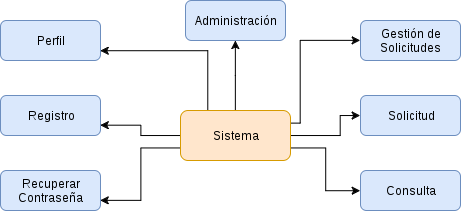
\includegraphics[width=\textwidth]{img/modulos_del_sistema.png}
\end{center}
\caption{Diagrama de módulos del sistema. Fuente:El Autor.}
\label{fig:Modulos_del_sistema}
\end{figure}


\textbf{Módulos}:
\begin{itemize}
	\item Administración: En este modulo el usuario con perfil administrador puede configurar parámetros referentes a los usuarios del sistema.
	
	\item Registro: En este modulo los usuarios pueden registrarse en este sistema ya sea como usuario tipo Inspectores o Taquilla.
	
	\item Perfil: Este modulo le permite al usuario modificar su información de contacto registrada en el sistema.
	
	\item Recuperar Contraseña: En este modulo los usuarios pueden recuperar su contraseña en caso de olvidarla. 
	
	\item Consulta: Este modulo hace énfasis en los filtros necesarios para la búsqueda de información dentro del sistema ya sea de solicitudes, usuarios o clientes (Aquellos que trajeron el carro a inspección)
	
	\item Solicitud: En este modulo los tipo de usuario Taquilla, al recibir un cliente, crean una solicitud de inspección.
	
	\item Gestión de Solicitudes: En este modulo los tipo de usuario Inspector realizan el registro de los datos de la inspección del vehículo y la gestión de las solicitudes de inspección.
	

\end{itemize}


\subsection{Interfaces de la aplicación}
\setlength{\parskip}{5mm}

\textbf{-Interfaz de inicio de sesión}: La figura a continuación muestra el formulario de inicio de sesión para aquellos usuarios registrados en el sistema.

\begin{figure}[H]
\begin{center}
	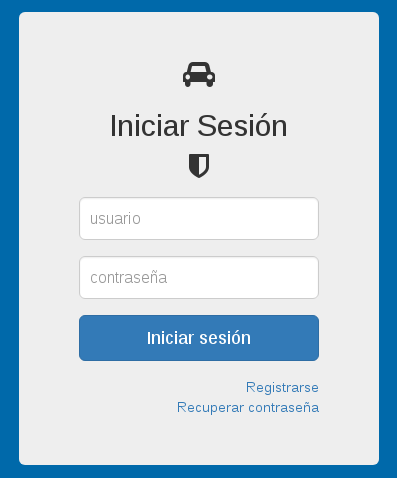
\includegraphics[width=8cm,height=10cm]{img/interfaces/inicio_sesion.png}
\end{center}
\caption{Interfaz de Inicio de Sesión. Fuente:Print Screen.}
\label{fig:interfaz_inicion_sesion}
\end{figure}

A partir de esta interfaz los usuarios registrados en el sistema podrán loguearse con su usuario y contraseña, en caso de no estar registrados se presenta la opción para registrarse, además se muestra la opción de recuperar contraseña en caso de que el usuario la haya olvidado

\textbf{-Interfaz de recuperar contraseña}: La figura a continuación muestra el formulario de recuperación de contraseña para aquellos usuarios registrados en el sistema.

%\begin{figure}
%\begin{center}
%	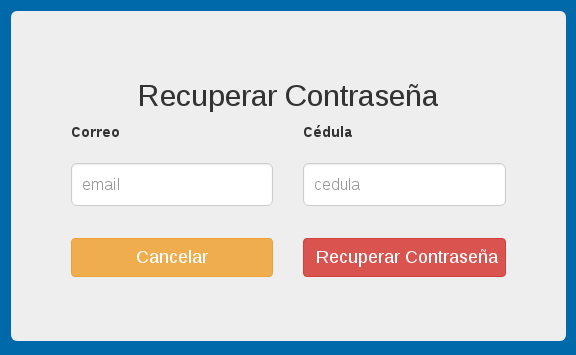
\includegraphics[width=14cm,height=8cm]{img/interfaces/recuperar_contrasena.png}
%\end{center}
%\caption{Interfaz de Recuperar Contraseña. Fuente:Print %Screen.}
%\label{fig:interfaz_recuperar_contraseña}
%\end{figure}

A partir de esta interfaz los usuarios registrados en el sistema podrán recuperar su contraseña mediante el formulario incluyendo su correo y cédula. Se generara una contraseña aleatoria que sera enviada a su correo con la cual podrán acceder al sistema, para luego cambiar su contraseña a una propia.


\textbf{-Interfaz registro de usuarios}: La figura a continuación muestra el formulario de registro de usuarios para aquellos usuarios no registrados en el sistema.

\begin{figure}[H]
\begin{center}
	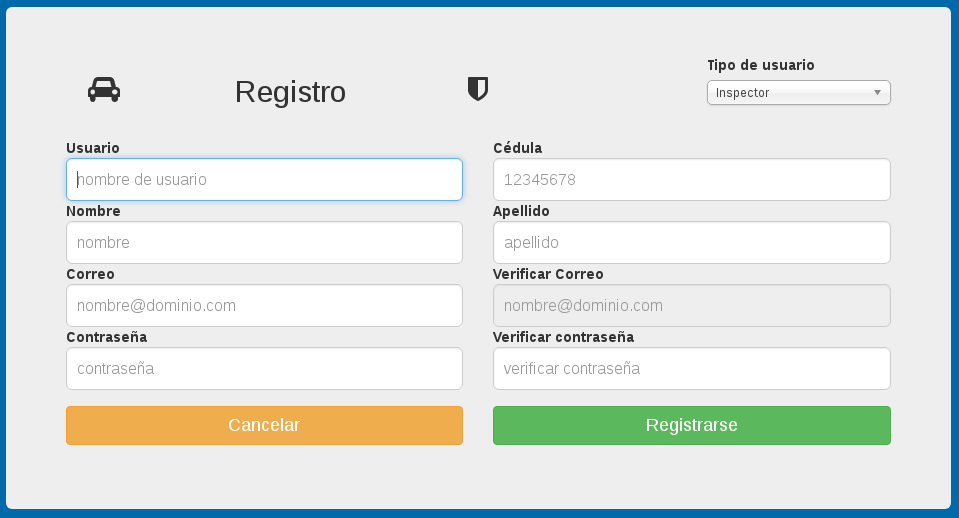
\includegraphics[width=14cm,height=8cm]{img/interfaces/registro_usuario.png}
\end{center}
\caption{Interfaz de Registro de Usuarios. Fuente:Print Screen.}
\label{fig:interfaz_registro_usuario}
\end{figure}

En esta interfaz los usuarios pueden registrarse bien sea como Inspectores o como usuarios Taquilla, ingresando su información personal.


\textbf{-Interfaz registro de usuarios}: La figura a continuación muestra el formulario de registro de usuarios para aquellos usuarios no registrados en el sistema.

\begin{figure}[H]
\begin{center}
	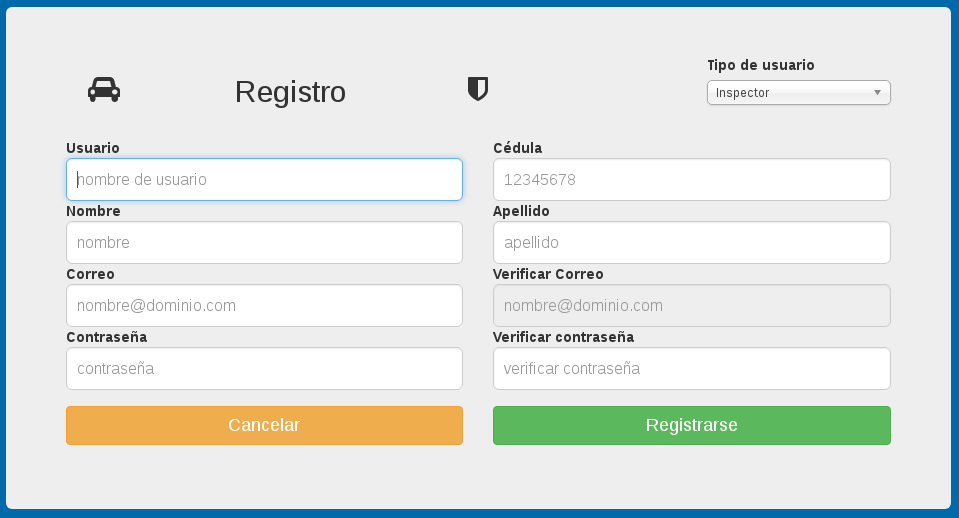
\includegraphics[width=14cm,height=8cm]{img/interfaces/registro_usuario.png}
\end{center}
\caption{Interfaz de Registro de Usuarios. Fuente:Print Screen.}
\label{fig:interfaz_registro_usuario}
\end{figure}

En esta interfaz los usuarios pueden registrarse bien sea como Inspectores o como usuarios Taquilla, ingresando su información personal.


\textbf{-Interfaz Configuración de Perfil }: La figura a continuación muestra el formulario de registro de usuarios para aquellos usuarios no registrados en el sistema.

\begin{figure}[H]
\begin{center}
	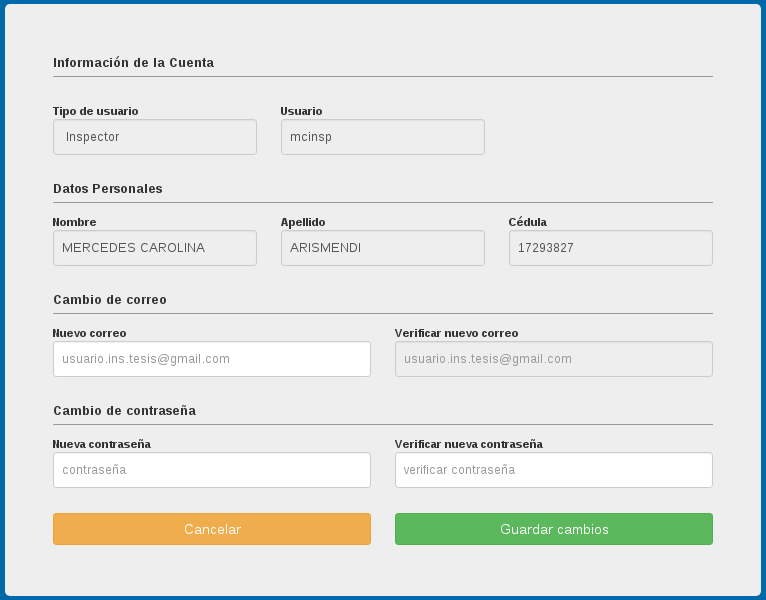
\includegraphics[width=12cm,height=8cm]{img/interfaces/editar_usuario.png}
\end{center}
\caption{Interfaz de Configuración del Perfil de Usuario. Fuente:Print Screen.}
\label{fig:interfaz_configuracion_usuario}
\end{figure}

En esta interfaz los usuarios pueden modificar su información personal ya sea el correo o contraseña.


\textbf{-Interfaz Administrador Edición de Usuarios }: La figura a continuación muestra el filtro y bandeja de los usuarios registrados en el sistema.

\begin{figure}[H]
\begin{center}
	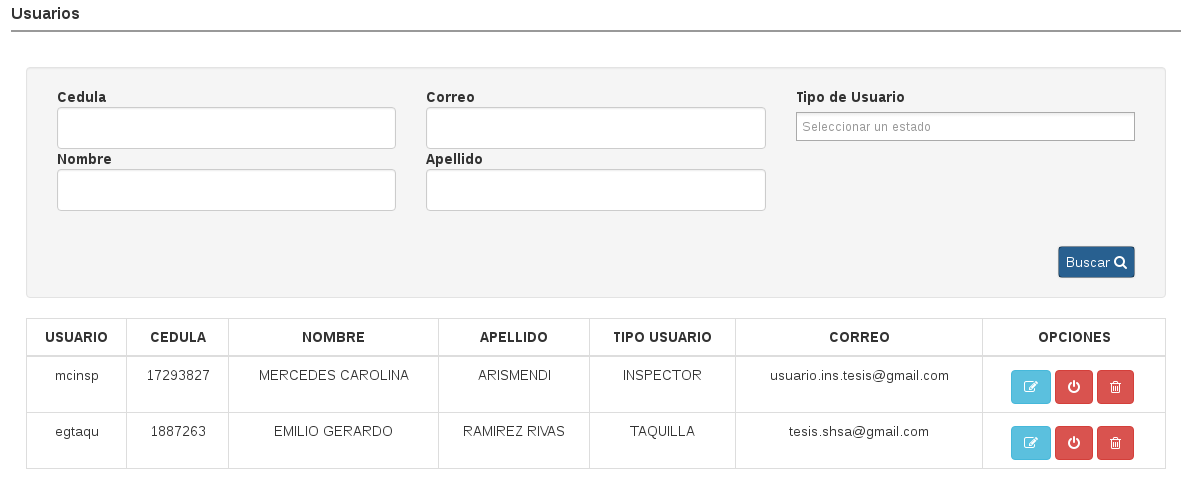
\includegraphics[width=\textwidth,height=7cm]{img/interfaces/bandeja_edicion_usuarios.png}
\end{center}
\caption{Interfaz de bandeja edición usuario por Administrador. Fuente:Print Screen.}
\label{fig:interfaz_bandeja_edicion_usuario}
\end{figure}

En esta interfaz los usuarios pueden ser modificados, inactivados y eliminados. Inactivados siempre y cuando no tengan una solicitud de inspección en proceso y eliminado siempre y cuando no tengan ninguna solicitud asociada al mismo.


\textbf{-Modal Inactivar Usuario }: La figura a continuación muestra el modal de confirmación para inactivar un usuario.

\begin{figure}[H]
\begin{center}
	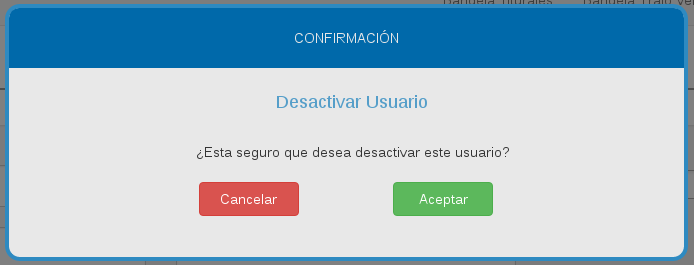
\includegraphics[width=14cm,height=6cm]{img/interfaces/modal_inactivar_usuario.png}
\end{center}
\caption{Modal Inactivar Usuario. Fuente:Print Screen.}
\label{fig:modal_confirmacion_inactivar_usuario}
\end{figure}

\textbf{-Modal Eliminar Usuario }: La figura a continuación muestra el modal de confirmación para eliminar un usuario.

\begin{figure}[H]
\begin{center}
	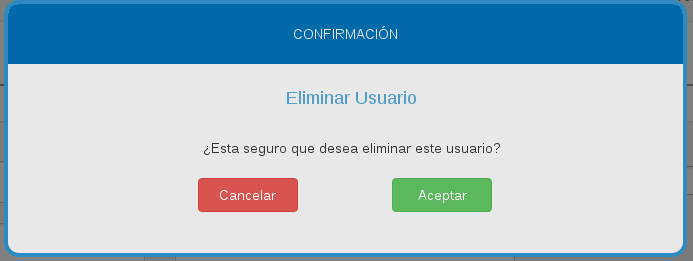
\includegraphics[width=14cm,height=6cm]{img/interfaces/modal_eliminar_usuario.png}
\end{center}
\caption{Modal Eliminar Usuario. Fuente:Print Screen.}
\label{fig:modal_confirmacion_eliminar_usuario}
\end{figure}





\setlength{\parskip}{0mm}




\section{Fase de pruebas maybe } 
\setlength{\parskip}{5mm}
\setlength{\parskip}{0mm}


\subsection{Pruebas funcionales}
\setlength{\parskip}{5mm}
\setlength{\parskip}{0mm}

\subsection{Pruebas de aceptación}
\setlength{\parskip}{5mm}
\setlength{\parskip}{0mm}
|
\chapter*{CONCLUSIÓN Y RECOMENDACIONES }

\addcontentsline{toc}{chapter}{CONCLUSIÓN Y RECOMENDACIONES}


\nocite{*}

\backmatter


\renewcommand{\bibname}{BIBLIOGRAFÍA}
\bibliographystyle{plainnat}
\bibliography{bibliografia.bib}

\end{document}